\documentclass[12pt]{article}
\usepackage[margin=1in]{geometry}
\usepackage{amsmath,amssymb,amsthm}
\usepackage{graphicx}
\usepackage{hyperref}
\usepackage{xcolor}
\usepackage{float}
\newlength\tindent
\setlength{\parindent}{0pt}
\setlength{\tindent}{\parindent}
\renewcommand{\indent}{\hspace*{\tindent}}


\usepackage{subcaption}

\title{Observability and State Estimation of a 2D Quadrotor System with Unknown Control Matrix \\ \large Project for Nonlinear and Data Driven Estimation}
\author{Tamzeed Elahi Toha}
\date{\today}



\begin{document}
\maketitle


Code for this project can be found \href{https://github.com/tamzeed-toha/Nonlinear_and_Data_Driven_Estimation/blob/main/project/phase_03.ipynb}{\textcolor{blue}{here}}.

\section*{Abstract}
In this project, I have analyzed the observability of a 2D quadrotor system with unknown control matrix. The complexity of the problem is mitigated by considering the unknown parameter as constants. The nonlinearity of the system makes the observability of system time-variant. To test it out, I have simulated the system's response with different sensory combinations and trajectories and measured their observability. Finally, the states of the system, along with the unknown parameters, are estimated using an Extended Kalman Filter. This project aims to achieve two objectives: a) estimating the unknown governing equations that relate inputs to the states; b) enhancing state estimations with the help of observability. The results found here will help in designing more observable state trajectories and in examining different behavioral motifs for biological systems. Where the translation of decisions to physical actions is often poorly understood.


\section*{Introduction}
Observability is an indication of the state quantities that can be "observed" from measurements. In the case of a linear system, it depends on both system and measurement matrices and is independent of time. But in the case of a nonlinear system, observability can be time dependent. That gives rise to an opportunity to design a more robust state estimator that takes advantage of the observability or plan trajectories that are more observable. In natural world, this nonlinearity leads to certain behavioral motifs which they use to improve state estimation. 

In this paper, I am going to investigate the behavior of a 2D quadrotor system with unknown control matrix. The necessity of knowing the control matrix beforehand to estimate state is often too restrictive for real-world applications. To combat that, researchers have proposed different strategies to estimate the unknown control matrix. In this paper \cite{Kong_2019}
, authors have proposed MRAC method with an adaptive law that converges to true control matrix, considering the system is time invariant. For the sake of relevence, I have used Extended Kalman Filter to estimate the unknown parameters of the control matrix. Figuring out the true dynamics of a system with more complicated control matrix is a much harder problem. I believe \cite{Brunton_2016} and other model discovery algorithms can be used to discover the true dynamics of the system. Although pySINDy is a powerful tool, its capability to estimate system dynamics even with a good set of prior knowledge is still inadequate.

To measure observability of the system, a few tools are used in this paper. First it is estimated analytically by calculating the rank of the observability matrix. As observability varies with state values, it is then measured with simulated data with a set of different trajectories. Lastly, the Emperical Observability Method with a small window size ($s=20$ timesteps) is used to estimate Cramer Rao Lower Bound of individual states. The results are compared across different measurement matrices and trajectories.

In this course, we have discussed two different estimators: Extended Kalman Filter and Unscented Kalman Filter. UKF being the more robust one, works by approximating the probability distribution of the states, whereas EKF works by linearizing the system dynamics by taking the first order Taylor expansion. Although UKF is better for nonlinear systems, it has proven to be more complicated to be implemented. For that reason, here I have used EKF for state estimation.



\section*{Analytical model of quadrotor system}
\begin{figure}[h!]
    \begin{subfigure}[t]{0.5\textwidth}
        \centering
        \includegraphics[width=5cm]{figures/model_diagram.png}
        \caption{Quadrotor system \cite{model_diagram}}
        \label{fig:1a}
    \end{subfigure}
    \hfill
    \begin{subfigure}[t]{0.5\textwidth}
        \centering
        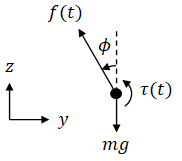
\includegraphics[width=5cm]{figures/free_body_diagram.png}
        \caption{Free body diagram \cite{model_diagram}}
        \label{fig:1b}
    \end{subfigure}
\end{figure}
% \includegraphics[width=5cm]{model_diagram.png}

The state space model of a quadrotor system can be found in various literature\cite{K2019}\cite{Schreier2012}. For the class project, I will be using a simplified 2D model (only the y and z coordinates). The dynamic equation of the system can be estimated using Newton's second law of motion.
\begin{align*}
    \ddot{y} &= -\frac{1}{m}u_1(t) \sin{\theta} \\
    \ddot{z} &= -g + \frac{1}{m}u_1(t) \cos{\theta} \\ 
    \ddot{\theta} &= \frac{1}{I_{xx}}u_2(t) \\
\end{align*}
I assumed only two inputs (force and torque) are present in the system. Although, their relation with the states are primarily nonlinear, it can be linearized with approximation $\phi \approx 0$. In future work, I will consider the rotor speeds as inputs to the system where the control matrix is more difficult to estimate but the input signals are much more reliable. \\\\
States are: $x = [\dot{\theta}, \theta, \dot{x}, x, \dot{z}, z]^T$ \\
inputs are:
\begin{align*}
    u_1(t) &= F \\
    u_2(t) &= \tau
\end{align*}
matrices in continuous form:
\begin{align*}
    A &= \begin{bmatrix}
        0 & 1 & 0 & 0 & 0 & 0 \\
        0 & 0 & 0 & 0 & 0 & 0 \\
        0 & 0 & 0 & 1 & 0 & 0 \\
        0 & 0 & 0 & 0 & 0 & 0 \\
        0 & 0 & 0 & 0 & 0 & 1 \\
        0 & 0 & 0 & 0 & 0 & 0
    \end{bmatrix} \\
    B &= \begin{bmatrix}
        0 & 0 \\
        0 & \frac{1}{I_{xx}} \\
        0 & 0 \\
        - \frac{1}{m} \sin{\theta} & 0 \\
        0 & 0 \\
        \frac{1}{m} \cos{\theta} & 0 \\
    \end{bmatrix} \\
\end{align*}


\section*{Results:}

\subsection*{Linear case:}
The nonlinearity of this system is due to the input matrix. The input matrix is a function of the states. So, the system is nonlinear. If we consider the unknown parameters of input matrix as a part of the state, then our new A matrix would be:

\begin{align*}
    \dot{x} &= \begin{bmatrix}
        0 & 1 & 0 & 0 & 0 & 0 & 0 & 0 & 0 \\
        0 & 0 & 0 & 0 & 0 & 0 & 0 & 0 & 0 \\
        0 & 0 & 0 & 1 & 0 & 0 & 0 & 0 & 0 \\
        0 & 0 & 0 & 0 & 0 & 0 & 0 & 0 & 0 \\
        0 & 0 & 0 & 0 & 0 & 1 & 0 & 0 & 0 \\
        0 & 0 & 0 & 0 & 0 & 0 & 0 & 0 & 0 \\
        0 & 0 & 0 & 0 & 0 & 0 & 0 & 0 & 0 \\
        0 & 0 & 0 & 0 & 0 & 0 & 0 & 0 & 0 \\
        0 & 0 & 0 & 0 & 0 & 0 & 0 & 0 & 0 \\
    \end{bmatrix} \begin{bmatrix}
        \dot{\theta} \\
        \theta \\
        \dot{x} \\
        x \\
        \dot{z} \\
        z \\
        \beta_1 \\
        \beta_2 \\
        \beta_3 \\
    \end{bmatrix} + \begin{bmatrix}
        0 & 0 \\
        0 & \frac{1}{I_{xx}} \\
        0 & 0 \\
        - \frac{1}{m} \sin{\theta} & 0 \\
        0 & 0 \\
        \frac{1}{m} \cos{\theta} & 0 \\
        0 & 0 \\
        0 & 0 \\
        0 & 0 \\
    \end{bmatrix} \begin{bmatrix}
        F \\
        \tau \\
    \end{bmatrix} 
\end{align*}

Our first task would be to estimate the unknown parameters of the input matrix knowing input matrix using an estimator (Kalman filter). As the A matrix is already linear, we have to discretize it first and then apply the Kalman filter. For our problem, lets break down the input matrix into two parts. One part is known and the other part is unknown.


\begin{align*}
    B_{n \times m} &= B^{0}_{n \times k} B^{1}_{k \times m} \\ 
    \text{so,}  \\
    \dot{x} &= Ax + B^{0} B^{1} u \\
    &= Ax + B^{0} u_{B} \\
    y &= Cx 
\end{align*}
where $B^{0}$ is unknown and $B^{1}$ is known. Here, $B^{0}$ is a row vector but it can be a matrix if the inputs are not linearly independent.

Contiuous form of the system:
\begin{align*}
    \dot{x} &= Ax + B^{0} u_{B} \\
    &= \begin{bmatrix}
        0 & 1 & 0 & 0 & 0 & 0 & 0 & 0 & 0 \\
        0 & 0 & 0 & 0 & 0 & 0 & 0 & 0 & 0 \\
        0 & 0 & 0 & 1 & 0 & 0 & 0 & 0 & 0 \\
        0 & 0 & 0 & 0 & 0 & 0 & 0 & 0 & 0 \\
        0 & 0 & 0 & 0 & 0 & 1 & 0 & 0 & 0 \\
        0 & 0 & 0 & 0 & 0 & 0 & 0 & 0 & 0 \\
        0 & 0 & 0 & 0 & 0 & 0 & 0 & 0 & 0 \\
        0 & 0 & 0 & 0 & 0 & 0 & 0 & 0 & 0 \\
        0 & 0 & 0 & 0 & 0 & 0 & 0 & 0 & 0 \\
    \end{bmatrix} \begin{bmatrix}
        \dot{\theta} \\
        \theta \\
        \dot{x} \\
        x \\
        \dot{z} \\
        z \\
        \beta_1 \\
        \beta_2 \\
        \beta_3 \\
    \end{bmatrix} + \begin{bmatrix}
        0 \\ \frac{1}{I_{xx}} \\ 0 \\ -\frac{1}{m} \\ 0 \\ \frac{1}{m} \\  0 \\ 0 \\ 0
        \end{bmatrix}^{T} \begin{bmatrix}
            0 & 0 \\
            0 & 1 \\
            0 & 0 \\
            \sin{\theta} & 0 \\
            0 & 0 \\
            \cos{\theta} & 0 \\
            0 & 0 \\
            0 & 0 \\
            0 & 0 \\
        \end{bmatrix} \begin{bmatrix}
            F \\
            \tau \\
        \end{bmatrix}
\end{align*}
We know, the continuous form of the system can be discretized using the following equation:
\begin{align*}
    A_d &= e^{A \Delta t}  = \phi(\Delta t) \\
    B_d &= (A_d - I) A^{-1} B \\
    C_d &= C
\end{align*}
In this case, A matrix is singular so we can't use the above equation. We can use the following equation to discretize the system:
\begin{align*}
    A_d &= I + A \Delta t + \frac{A^2 \Delta t^2}{2} + \frac{A^3 \Delta t^3}{6} + \ldots \\
    B_d &= \int_{0}^{\Delta t} e^{A \tau} d\tau B \\
    C_d &= C
\end{align*}
The discretized form of the system is:
\begin{align*}
    A_d &= \begin{bmatrix}
        1 & \Delta t & 0 & 0 & 0 & 0 & 0 & 0 & 0 \\
        0 & 1 & 0 & 0 & 0 & 0 & 0 & 0 & 0 \\
        0 & 0 & 1 & \Delta t & 0 & 0 & 0 & 0 & 0 \\
        0 & 0 & 0 & 1 & 0 & 0 & 0 & 0 & 0 \\
        0 & 0 & 0 & 0 & 1 & \Delta t & 0 & 0 & 0 \\
        0 & 0 & 0 & 0 & 0 & 1 & 0 & 0 & 0 \\
        0 & 0 & 0 & 0 & 0 & 0 & 1 & 0 & 0 \\
        0 & 0 & 0 & 0 & 0 & 0 & 0 & 1 & 0 \\
        0 & 0 & 0 & 0 & 0 & 0 & 0 & 0 & 1 \\
    \end{bmatrix} \\
\end{align*}


\color{black}
Estimation of $B_d$ matrix is a bit tricky because of the singularity of the A matrix. I have estimated the B matrix in two methods:
\begin{enumerate}
    \item Using pseudo-inverse (Moore-Penrose inverse) I got a zero matrix.
    \item Using the integral equation, I got a non-zero matrix. For $\Delta t = 0.1$, the B matrix is: $B_d = \begin{bmatrix}   6.25e-01 \\  1.25e+01 \\ -1.00e-02 \\ -2.00e-01 \\ 1.00e-02 \\ 2.00e-01 \\
        0.00e+00 \\  0.00e+00 \\  0.00e+00 \end{bmatrix}$
\end{enumerate}

\color{black}



Now, we divert our attention to the measurement matrix of the system. The observability of the system is dependent on the measurement matrix. We have to design the measurement matrix in such a way that the system is observable. 

\subsubsection*{Observability}
The observability of the system can be evaluated using the observability matrix. The system is observable if the rank of the observability matrix is equal to the number of states. The observability matrix is given by:
\begin{align*}
    O = \begin{bmatrix}
        C \\
        CA \\
        CA^2 \\
        \vdots \\
        CA^{n-1}
    \end{bmatrix}
\end{align*}

\subsection*{Designing a measurement matrix}
Let's consider the measurement matrix as an identity matrix. 
\begin{align*}
    C &= I
\end{align*}
This makes the system observable (rank = 9). We can get by with lower number of sensors. But, as the beta values don't really have a dynamics, they need direct measurement for estimation. At least for the linear case.

The measurement plot is given below:
\begin{figure}[h!]
    \centering
    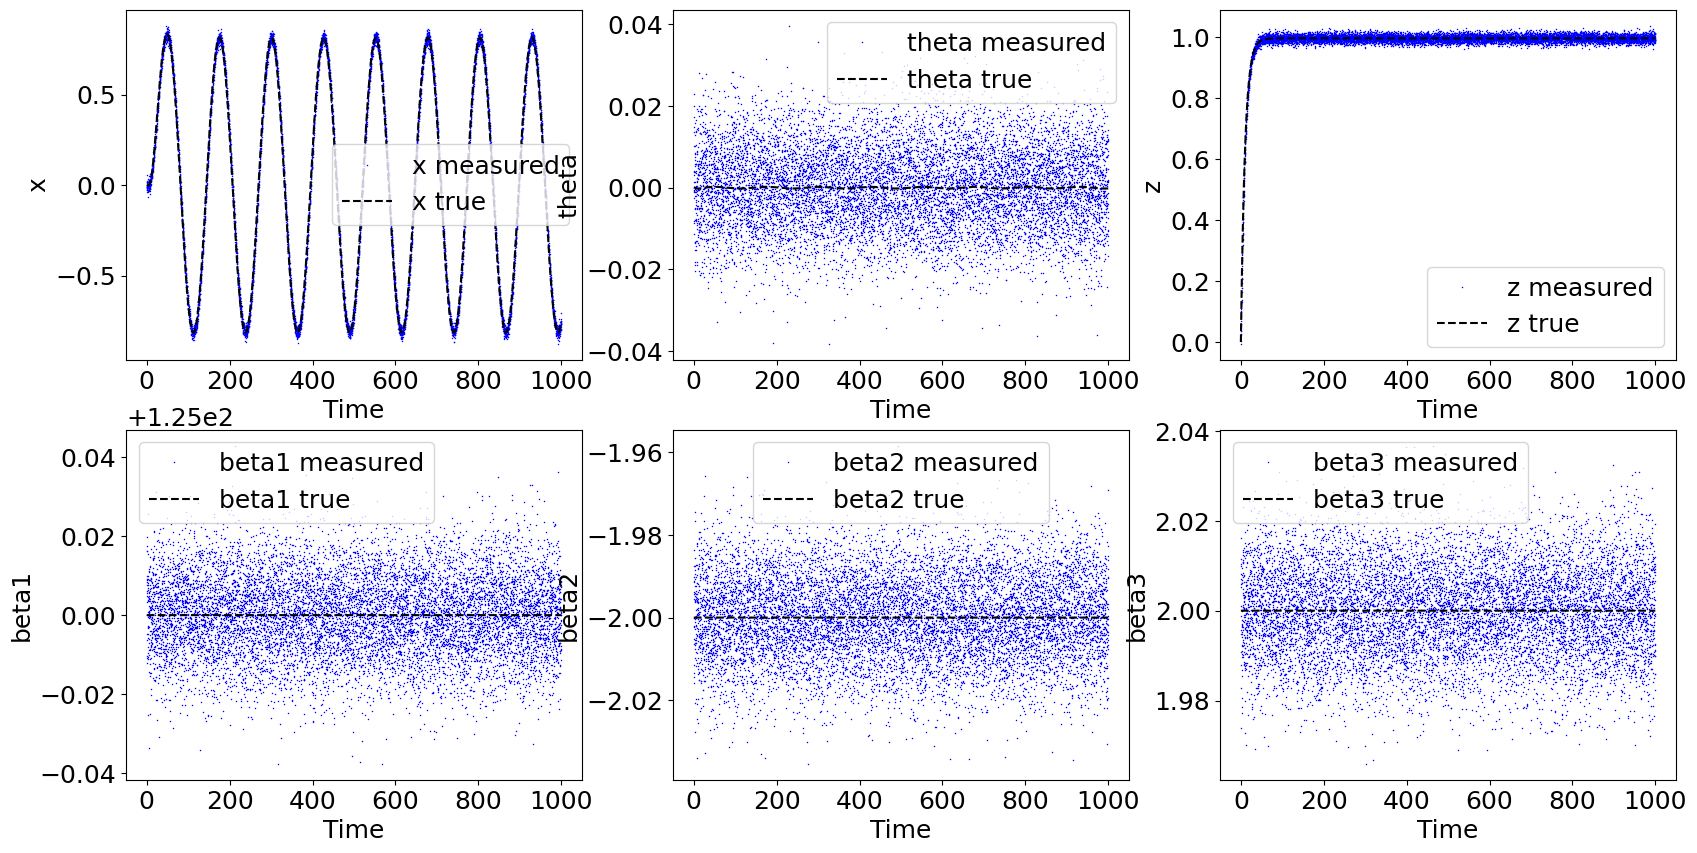
\includegraphics[width=10cm]{figures/phase_02_measurement1.png}
    \caption{Measurement plot}
    \label{fig:02}
\end{figure}
The estimator was able to estimate the states and the unknown parameters of the input matrix. The plot of the estimated states and the true states are given below:
\begin{figure}[h!]
    \centering
    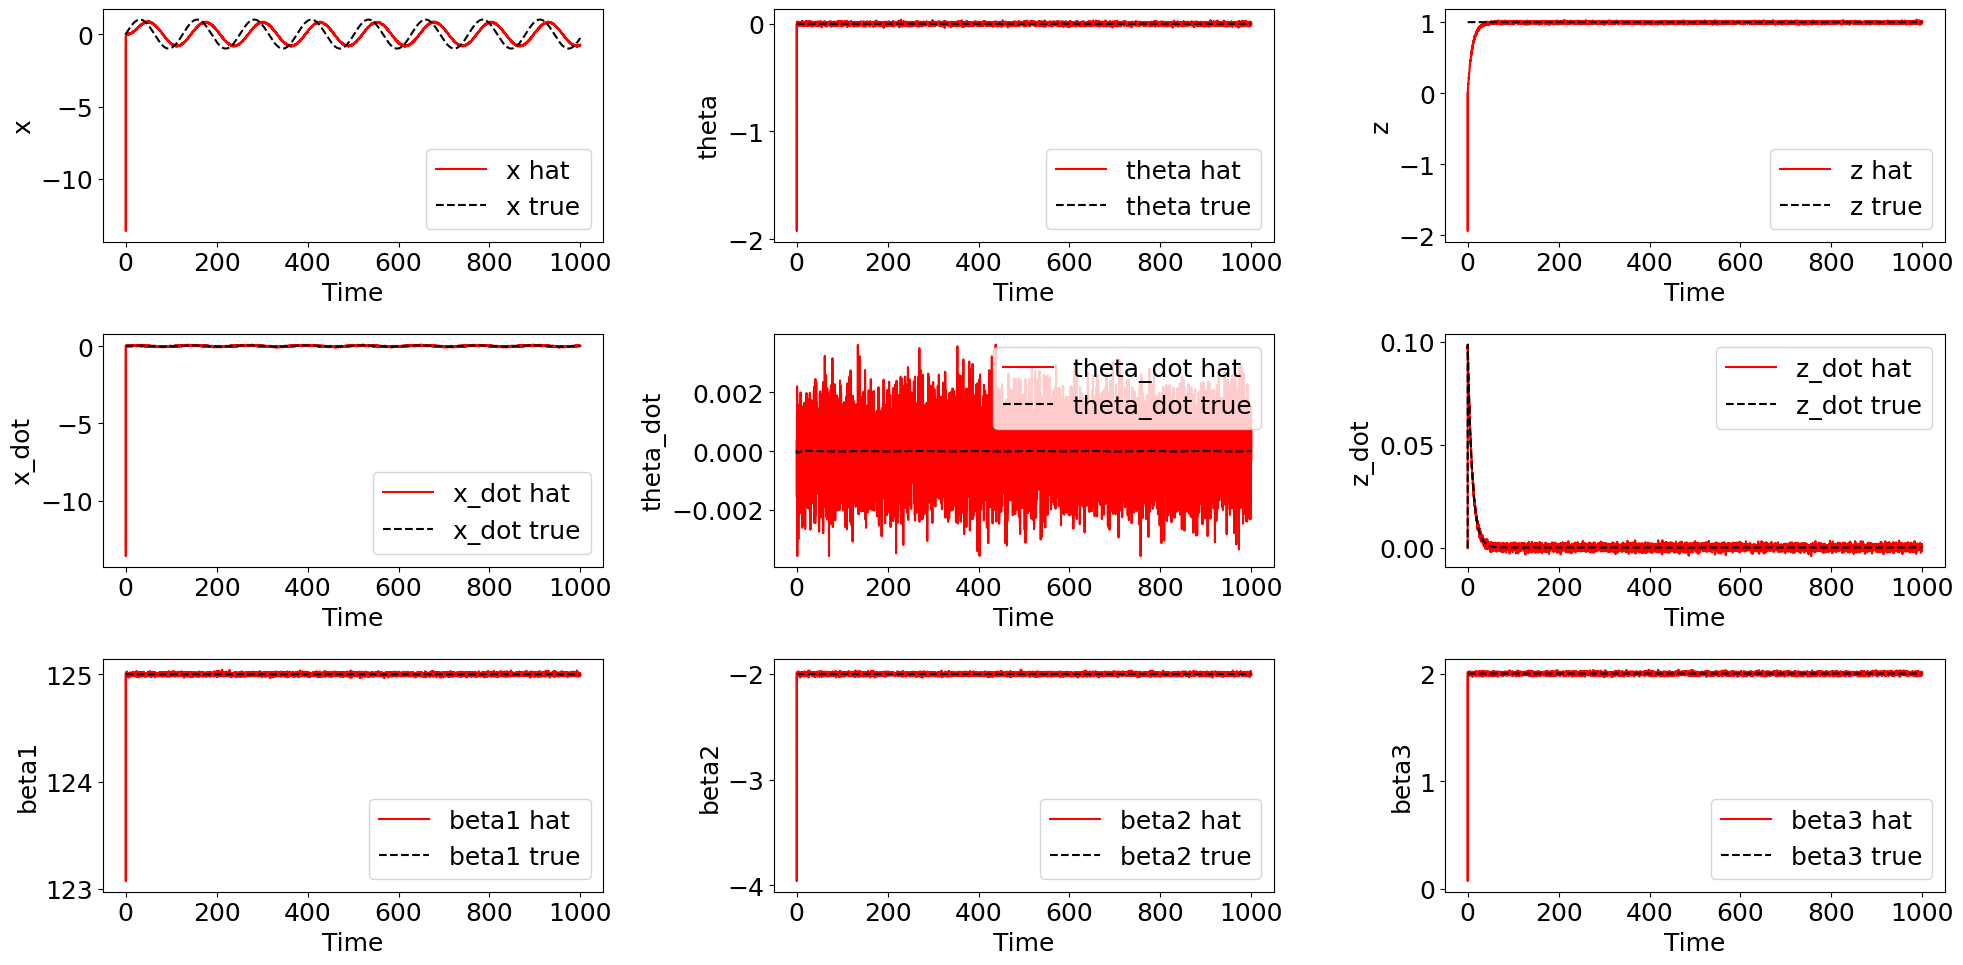
\includegraphics[width=10cm]{figures/phase_02_states1.png}
    \caption{State estimation}
    \label{fig:03}
\end{figure}

\subsection*{Nonlinear case:}
Now lets concentrate our attention to the nonlinear case. The system is nonlinear because it has unknown parameters in the input matrix (and also in the state matrix).  

\section*{Organized dynamic equations:}

States:
\begin{align*}
    \vec{x} &= \begin{bmatrix}
        \colorbox{yellow}{$\dot{\theta}$} \\
        \colorbox{yellow}{$\theta$} \\
        \colorbox{yellow}{$\dot{x}$} \\
        \colorbox{yellow}{$x$} \\
        \colorbox{yellow}{$\dot{z}$} \\
        \colorbox{yellow}{$z$} \\
        \hline
        \colorbox{pink}{$\beta_1$} \\
        \colorbox{pink}{$\beta_2$} \\
        % \colorbox{pink}{$\beta_3$} \\
    \end{bmatrix}
\end{align*}

Dynamic equations:
\begin{align*}
    \dot{\vec{x}} &= \begin{bmatrix}
        \colorbox{yellow}{$\dot{x_1}$} \\
        \colorbox{yellow}{$\dot{x_2}$} \\
        \colorbox{yellow}{$\dot{x_3}$} \\
        \colorbox{yellow}{$\dot{x_4}$} \\
        \colorbox{yellow}{$\dot{x_5}$} \\
        \colorbox{yellow}{$\dot{x_6}$} \\
        \hline
        \colorbox{pink}{$\dot{x_7}$} \\
        \colorbox{pink}{$\dot{x_8}$} \\
        % \colorbox{pink}{$\dot{x_9}$} \\
    \end{bmatrix} = \begin{bmatrix}
        1/I_{xx} \colorbox{green}{$u_2$} \\ 
        \colorbox{yellow}{$x_1$} \\
        1/m \colorbox{green}{$u_1$} \sin{\colorbox{yellow}{$x_2$}} \\
        \colorbox{yellow}{$x_3$} \\
        -g + 1/m \colorbox{green}{$u_1$} \cos{\colorbox{yellow}{$x_2$}} \\
        \colorbox{yellow}{$x_6$} \\
        \hline
        0 \\
        0 \\
        % 0 \\
    \end{bmatrix} = \begin{bmatrix}
        \colorbox{pink}{$x_7$} \colorbox{green}{$u_2$} \\
        \colorbox{yellow}{$x_1$} \\
        \colorbox{pink}{$x_8$} \colorbox{green}{$u_1$} \sin{\colorbox{yellow}{$x_2$}} \\
        \colorbox{yellow}{$x_3$} \\
        -\colorbox{cyan}{g} + \colorbox{pink}{$x_8$} \colorbox{green}{$u_1$} \cos{\colorbox{yellow}{$x_2$}} \\
        \colorbox{yellow}{$x_6$} \\
        \hline
        0 \\
        0 \\
        % 0 \\
    \end{bmatrix} \\
    &= \begin{bmatrix}
        0 \\
        \colorbox{yellow}{$x_1$} \\
        0 \\
        \colorbox{yellow}{$x_3$} \\
        -\colorbox{cyan}{g} \\
        \colorbox{yellow}{$x_6$} \\
        \hline
        0 \\
        0 \\
        % 0 \\
        \end{bmatrix} + \begin{bmatrix}
        0 \\
        0 \\
        \colorbox{pink}{$x_8$} \sin{\colorbox{yellow}{$x_2$}} \\
        0 \\
        \colorbox{pink}{$x_8$} \cos{\colorbox{yellow}{$x_2$}} \\
        0 \\
        \hline
        0 \\
        0 \\
        % 0 \\
    \end{bmatrix} \colorbox{green}{$u_1$} + \begin{bmatrix}
        \colorbox{pink}{$x_7$} \\
        0 \\
        0 \\
        0 \\
        0 \\
        0 \\
        \hline
        0 \\
        0 \\
        % 0 \\
    \end{bmatrix} \colorbox{green}{$u_2$} \\    
    &= \begin{bmatrix}
        0 \\
        \colorbox{yellow}{$\dot{\theta}$} \\
        0 \\
        \colorbox{yellow}{$\dot{x}$} \\
        -\colorbox{cyan}{g} \\
        \colorbox{yellow}{$\dot{z}$} \\
        \hline
        0 \\
        0 \\
        % 0 \\
    \end{bmatrix} +  \begin{bmatrix}
        0 \\
        0 \\
        % \colorbox{pink}{$\beta_2$} \\
        \colorbox{pink}{$x_8$} \\
        0 \\
        % \colorbox{pink}{$\beta_3$} \\
        \colorbox{pink}{$x_8$} \\
        0 \\
        \hline
        0 \\
        0 \\
        % 0 \\
    \end{bmatrix} \colorbox{lime}{$\tilde{u}_1$} + \begin{bmatrix}
        % \colorbox{pink}{$\beta_1$} \\
        \colorbox{pink}{$x_7$} \\
        0 \\
        0 \\
        0 \\
        0 \\
        0 \\ 
        \hline
        0 \\
        0 \\
        % 0 \\
    \end{bmatrix} \colorbox{lime}{$u_2$} \\
    &= f_0(\vec{x}) + f_1(\vec{x}) \tilde{u}_1 + f_2(\vec{x}) u_2
\end{align*}

where, 
\begin{align*}
    \tilde{u}_1 &= \begin{bmatrix}
        0 \\
        0 \\
        % \sin{\colorbox{yellow}{$\theta$}} \\
        \sin{\colorbox{yellow}{$x_2$}} \\
        0 \\
        % \cos{\colorbox{yellow}{$\theta$}} \\
        \cos{\colorbox{yellow}{$x_2$}} \\
        0 \\
        \hline
        0 \\
        0 \\
        % 0 \\
    \end{bmatrix} u_1
\end{align*}

known constants: \colorbox{cyan}{$g$} = 9.81 $m/s^2$ \\

Measurement matrix: I have played around with different measurement matrices and trajectories. Observability analysis and state estimation for all those measurements are given below.
\begin{align*}
    h &= \left[\begin{matrix}\dot{\theta}\\\theta\\\dot{x}\\x\\\dot{z}\\z\\\beta_{1}\\\beta_{2}\\\beta_{3}\end{matrix}\right], 
    \left[\begin{matrix}\theta\\x\\z\end{matrix}\right],
    \left[\begin{matrix}\theta\\x\end{matrix}\right], 
    \left[\begin{matrix}\theta x z\end{matrix}\right], 
    \left[\begin{matrix}\theta\\x z\end{matrix}\right],
    \left[\begin{matrix}\theta\\x + z\\z\end{matrix}\right],
    \left[\begin{matrix}\theta + x\\x + z\end{matrix}\right],
    \left[\begin{matrix}\theta + x\\x + z\\\theta + z\end{matrix}\right],
    \left[\begin{matrix}\theta x\\\frac{z}{x}\\\theta + z\end{matrix}\right],
    \left[\begin{matrix}\theta x\\\frac{z}{x}\end{matrix}\right],
    \left[\begin{matrix}\dot{\theta}\\\dot{x}\\\dot{z}\end{matrix}\right],
    \left[\begin{matrix}\dot{\theta}\\\theta\\\dot{x}\\\dot{z}\end{matrix}\right],
    \left[\begin{matrix}\dot{\theta}\\\log{\left(\theta \right)}\\\dot{x}\\\dot{z}\end{matrix}\right]
\end{align*}

\subsection*{Observability analysis:}
First, the observability of this nonlinear system is estimated analytically.The process involves taking the Lie derivative of the system dynamics with respect to the states and generating the G matrix. Observability matrix can be found by taking the jacobian of the G matrix. The rank of the observability matrix if greater than the number of states, makes the system observable. Analytically we see the systems with direct measurements of each degree of freedom are full rank \ref{fig:04a}. To check if the observability is time variant, I have plotted the observability of different measurements and trajectories with time \ref{fig:04b}. Unfortunately, it is found to be not time variant. But we move on to the emperical observability analysis.

Emperical observability measures relative excitation of states with respect to the inputs. In this case, I found the Cramer Rao Lower Bound of states are quite satisfactory though the condition number of the system is unnaturally high \ref{fig:04c}\ref{fig:04d}. One of the state might be unobservable in these scenarios and that might affect the condition number. The noise in Cramer Rao Bound is related to the perturbation of initial states. Initially I assumed the poor condition number value results from insufficient excitation of the states. But, upon further investigation, I found the condition number is high because the eigenvalue of one of the states is very high compared to other. This is further illustrated with figure \ref{supfig:01c}.

\begin{figure}[H]
    \begin{subfigure}[t]{\textwidth}
        \centering
        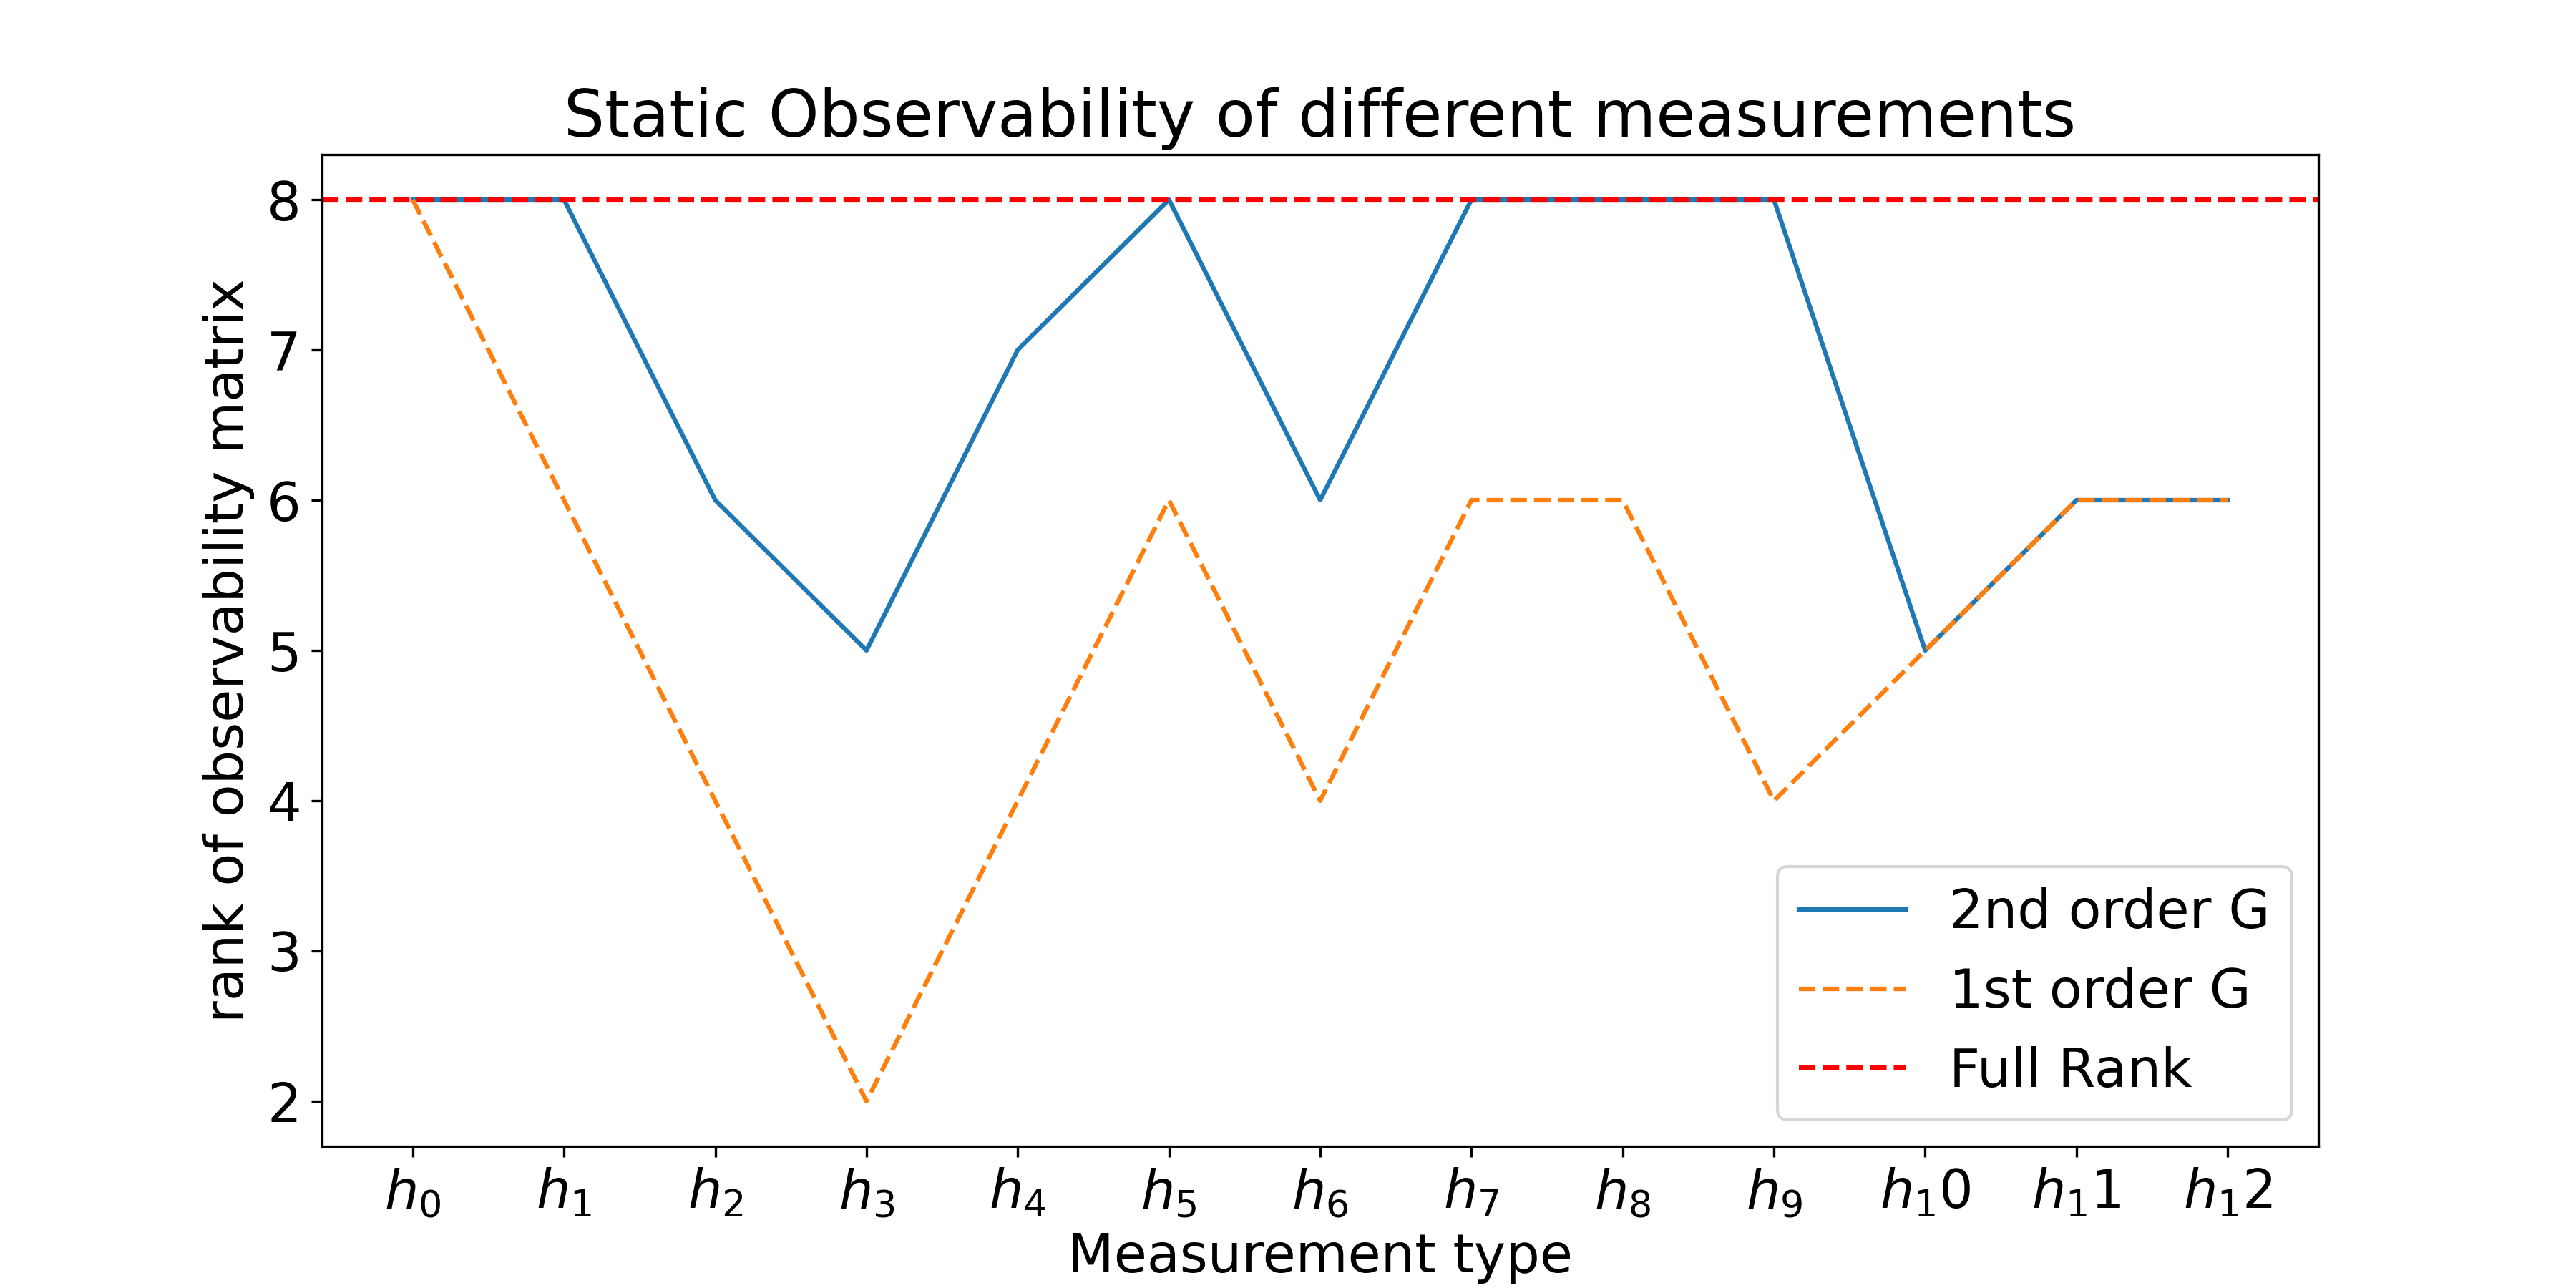
\includegraphics[width=10cm]{figures/analytical_observability.png}
        \caption{Analytical observability of different measurements matrices}
        \label{fig:04a}
    \end{subfigure}
    \\
    \begin{subfigure}[t]{\textwidth}
        \centering
        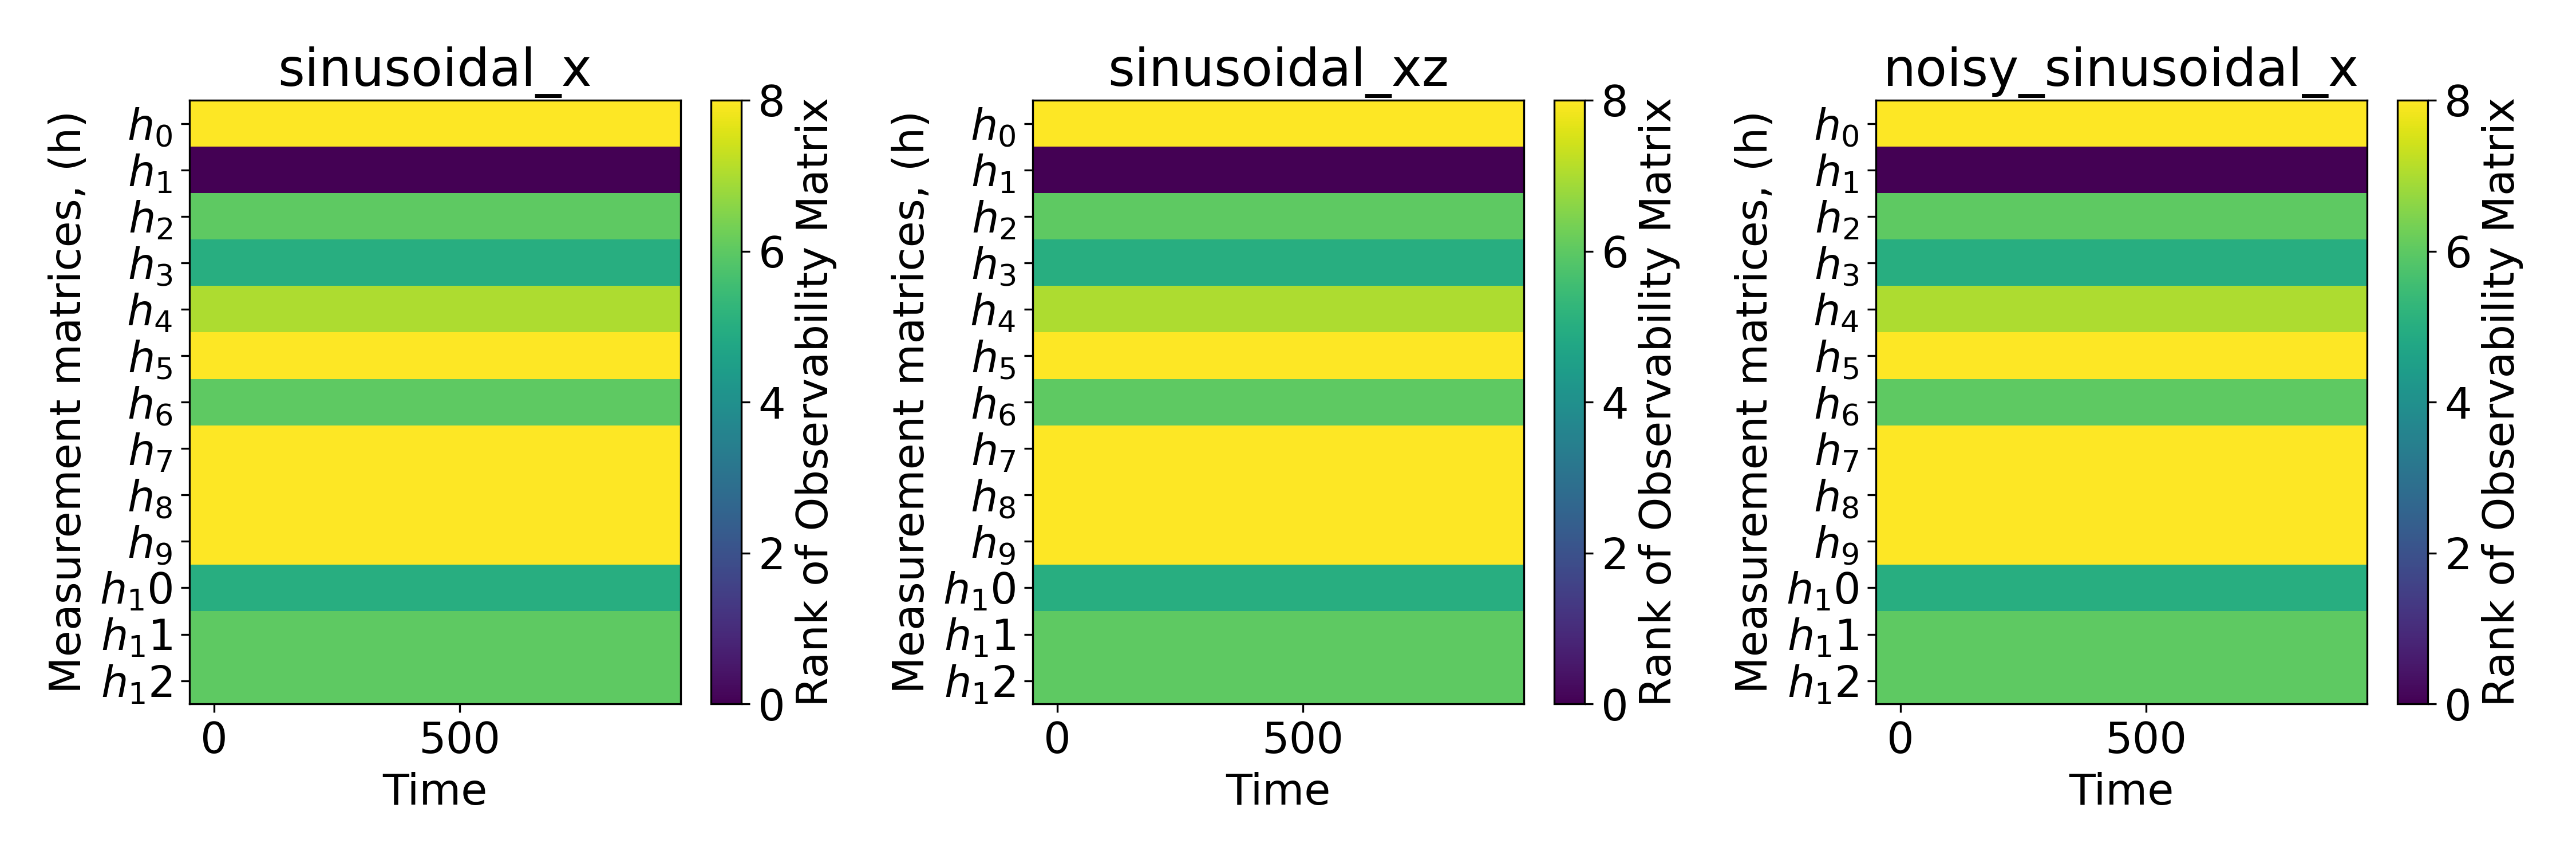
\includegraphics[width=15cm]{figures/observability_with_time.png}
        \caption{Observability of the system with time and measurement matrices}
        \label{fig:04b}
    \end{subfigure}
    \\
    \begin{subfigure}[t]{\textwidth}
        \centering
        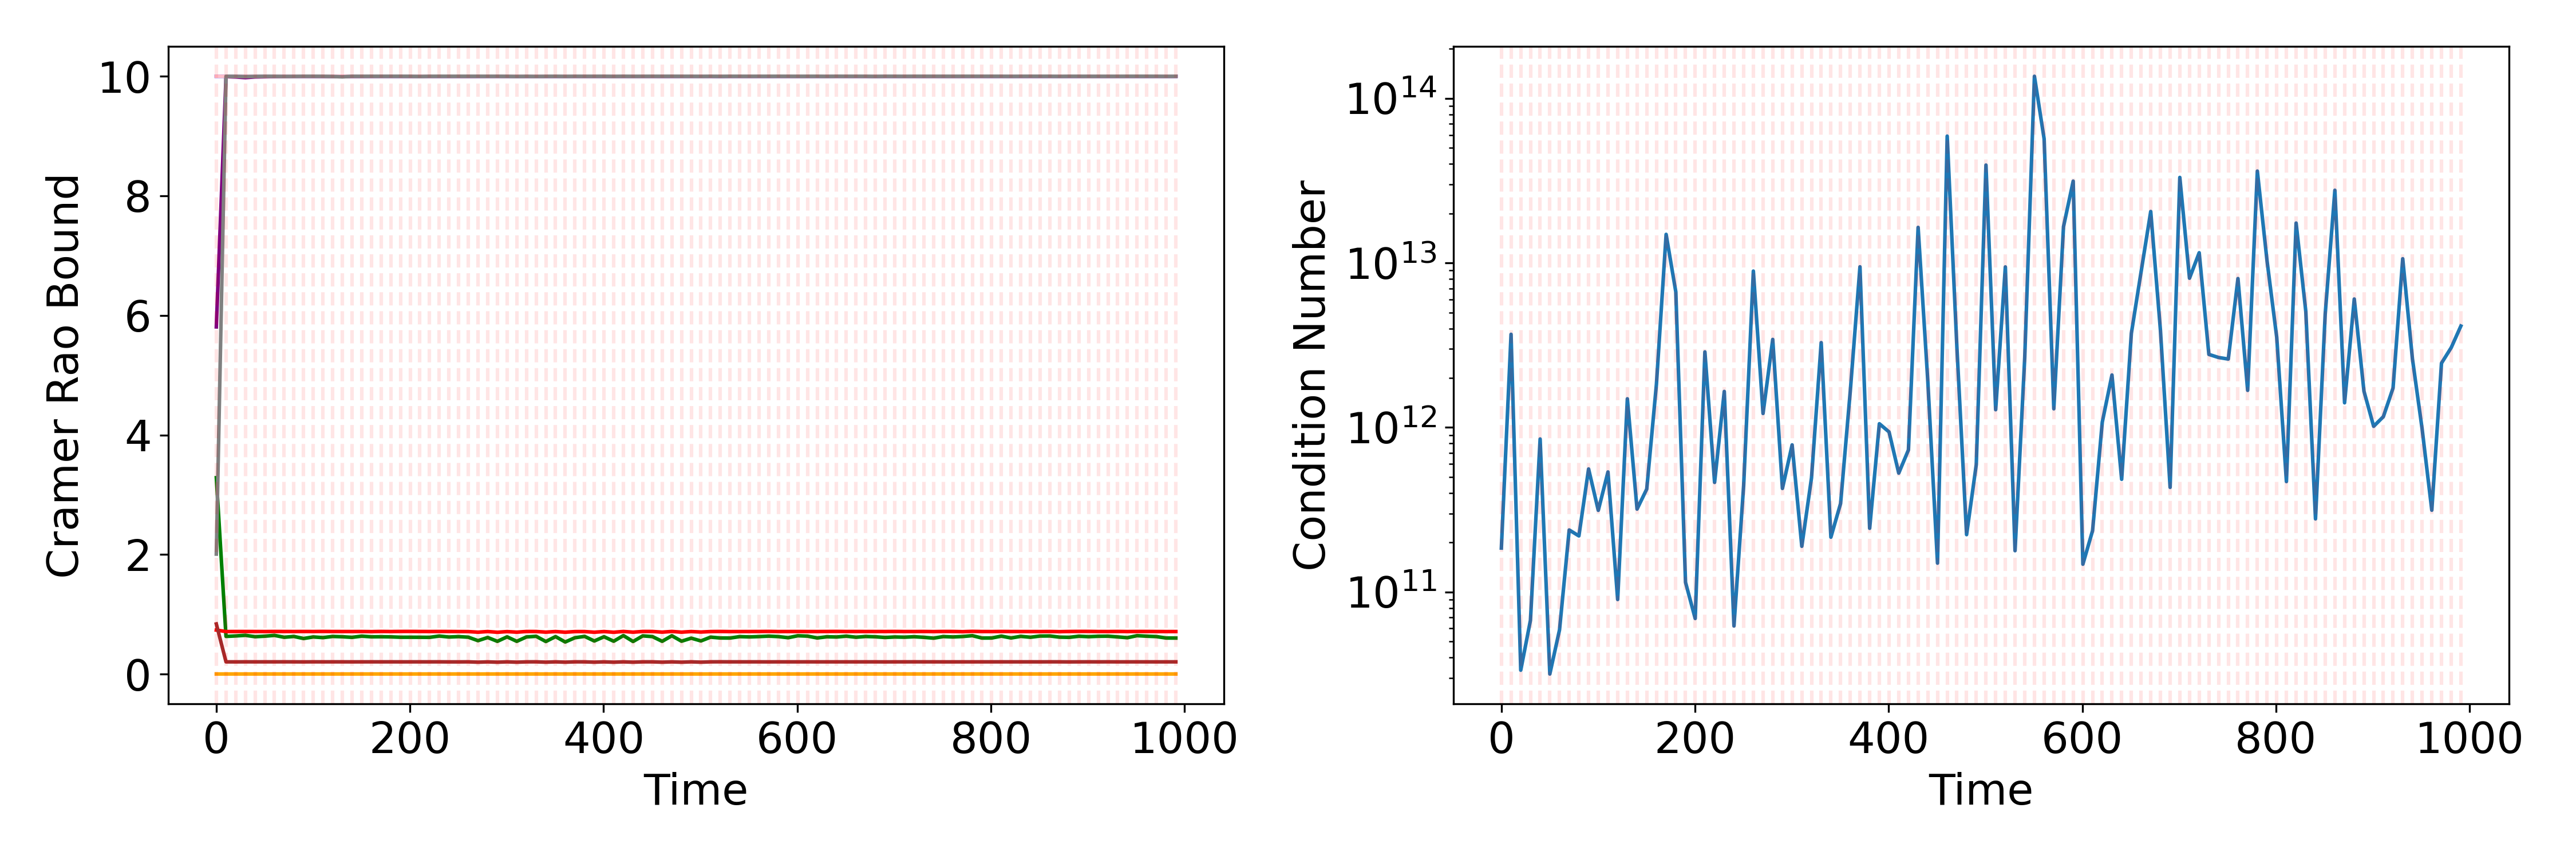
\includegraphics[width=15cm]{figures/crb_and_cn_with_noisy_sinusoidal_x_and_h1.png}
        \caption{Cramer Rao Lower Bound and Condition Number of the system with h1 measurement matrix}
        \label{fig:04c}
    \end{subfigure}
    \\
    \begin{subfigure}[t]{\textwidth}
        \centering
        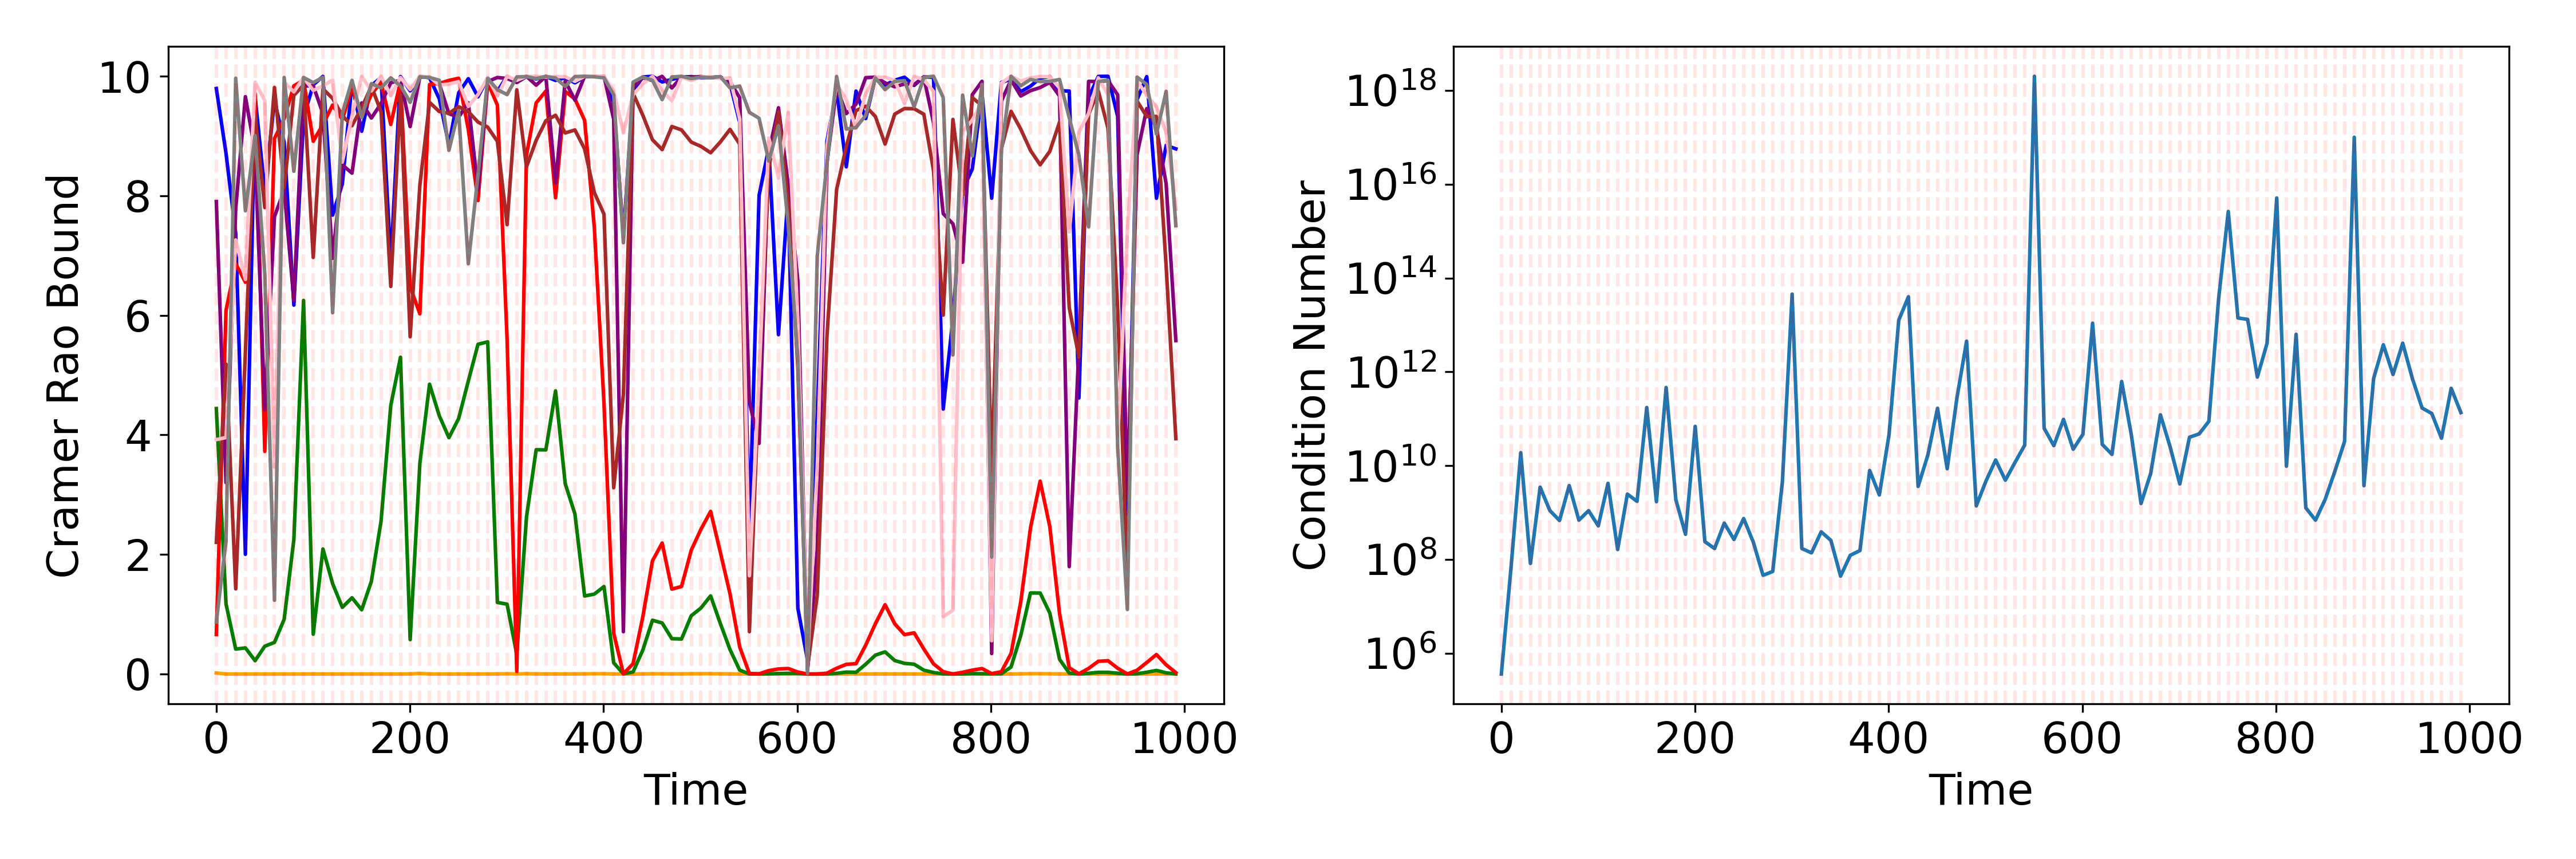
\includegraphics[width=15cm]{figures/crb_and_cn_with_noisy_sinusoidal_x_and_h9.png}
        \caption{Cramer Rao Lower Bound and Condition Number of the system with h9 measurement matrix}
        \label{fig:04d}
    \end{subfigure}
\end{figure}
Results from other measurement matrices along with the state values can be found in the supplementary material.


\subsection*{State estimation:}
Extended Kalman Filter is used to estimate the states of the system. The state estimation is done with different measurement matrices and trajectories. The results are given below for a few measurement matrices. 

\begin{figure}[H]
    \begin{subfigure}[t]{\textwidth}
        \centering
        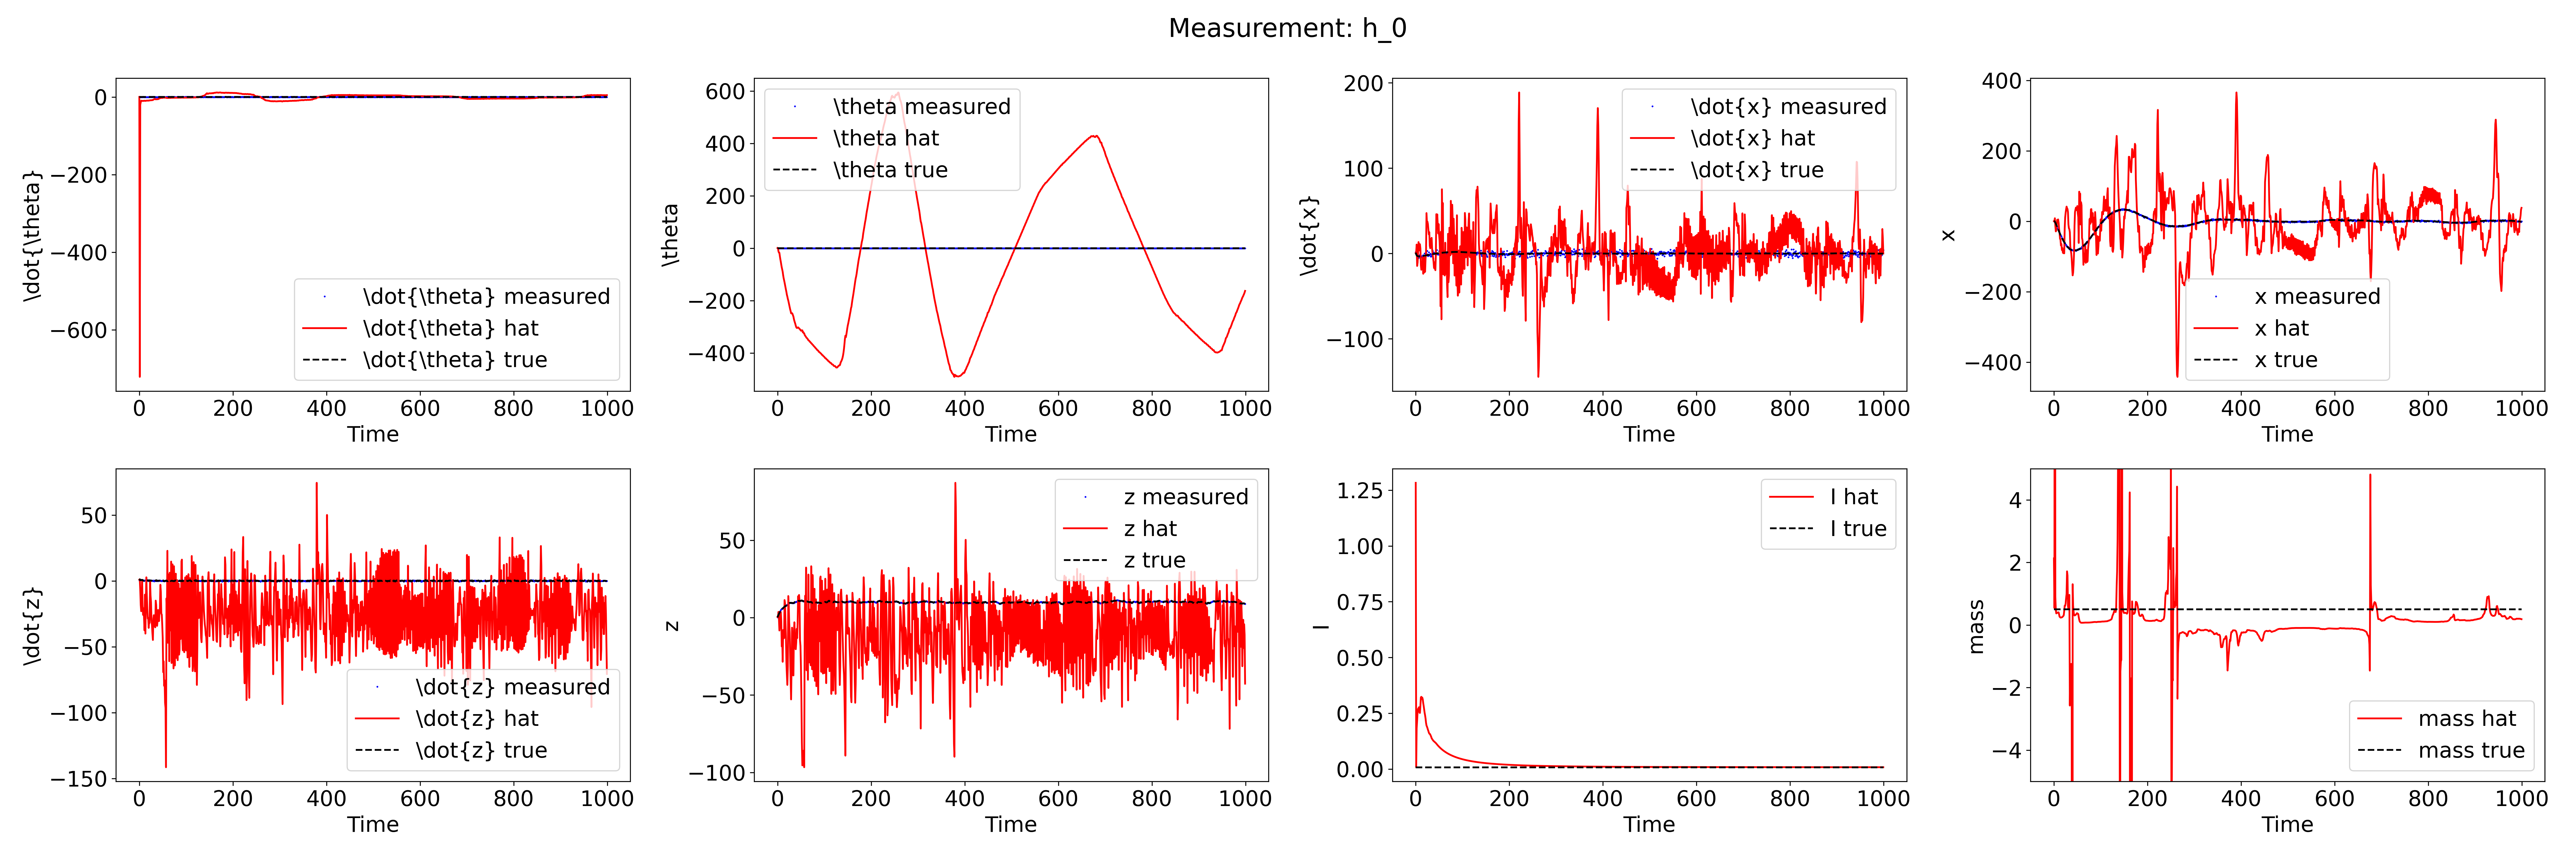
\includegraphics[width=15cm]{figures/ekf_with_noisy_sinusoidal_x_and_h0.png}
        \caption{State estimation with h0 measurement matrix}
        \label{fig:05a}
    \end{subfigure}
    \\
    \begin{subfigure}[t]{\textwidth}
        \centering
        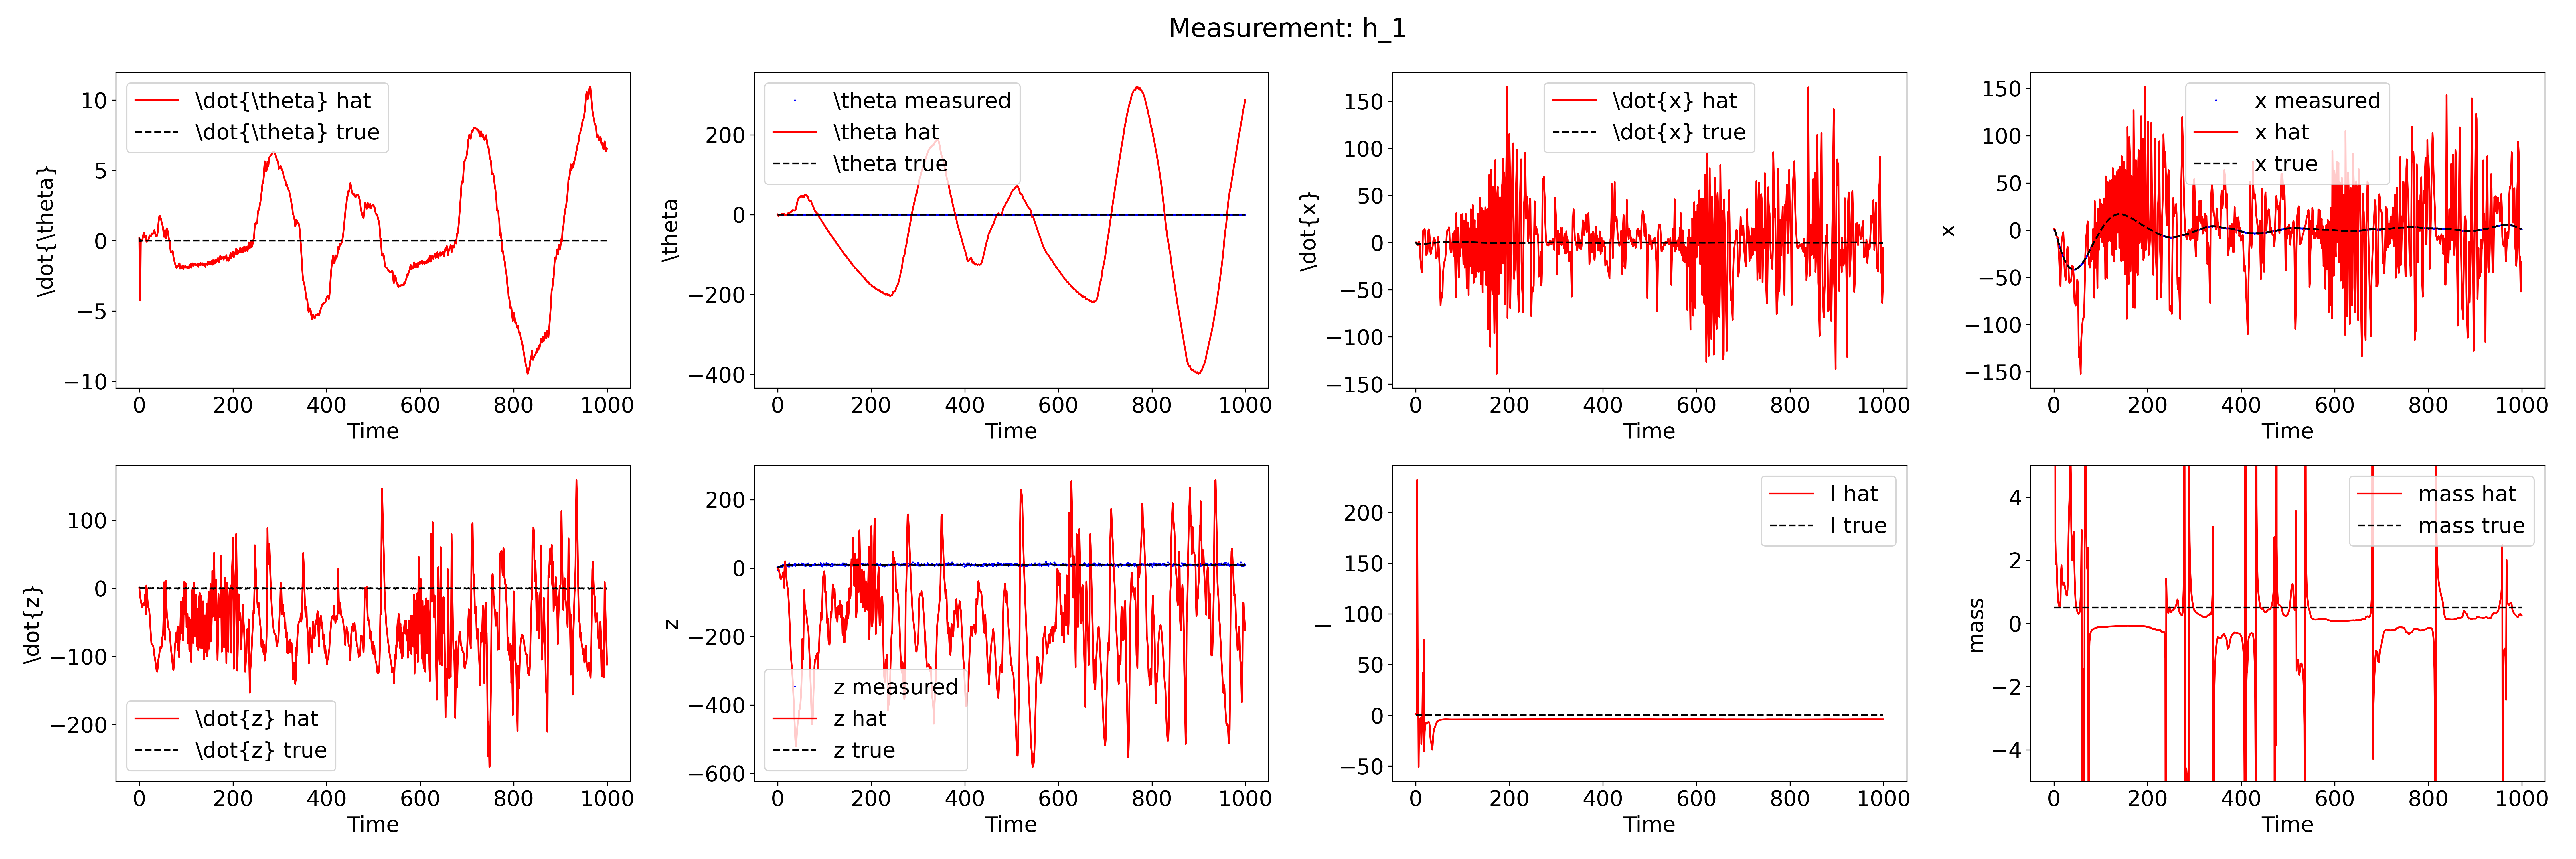
\includegraphics[width=15cm]{figures/ekf_with_noisy_sinusoidal_x_and_h1.png}
        \caption{State estimation with h1 measurement matrix}
        \label{fig:05b}
    \end{subfigure}
    \\
    \begin{subfigure}[t]{\textwidth}
        \centering
        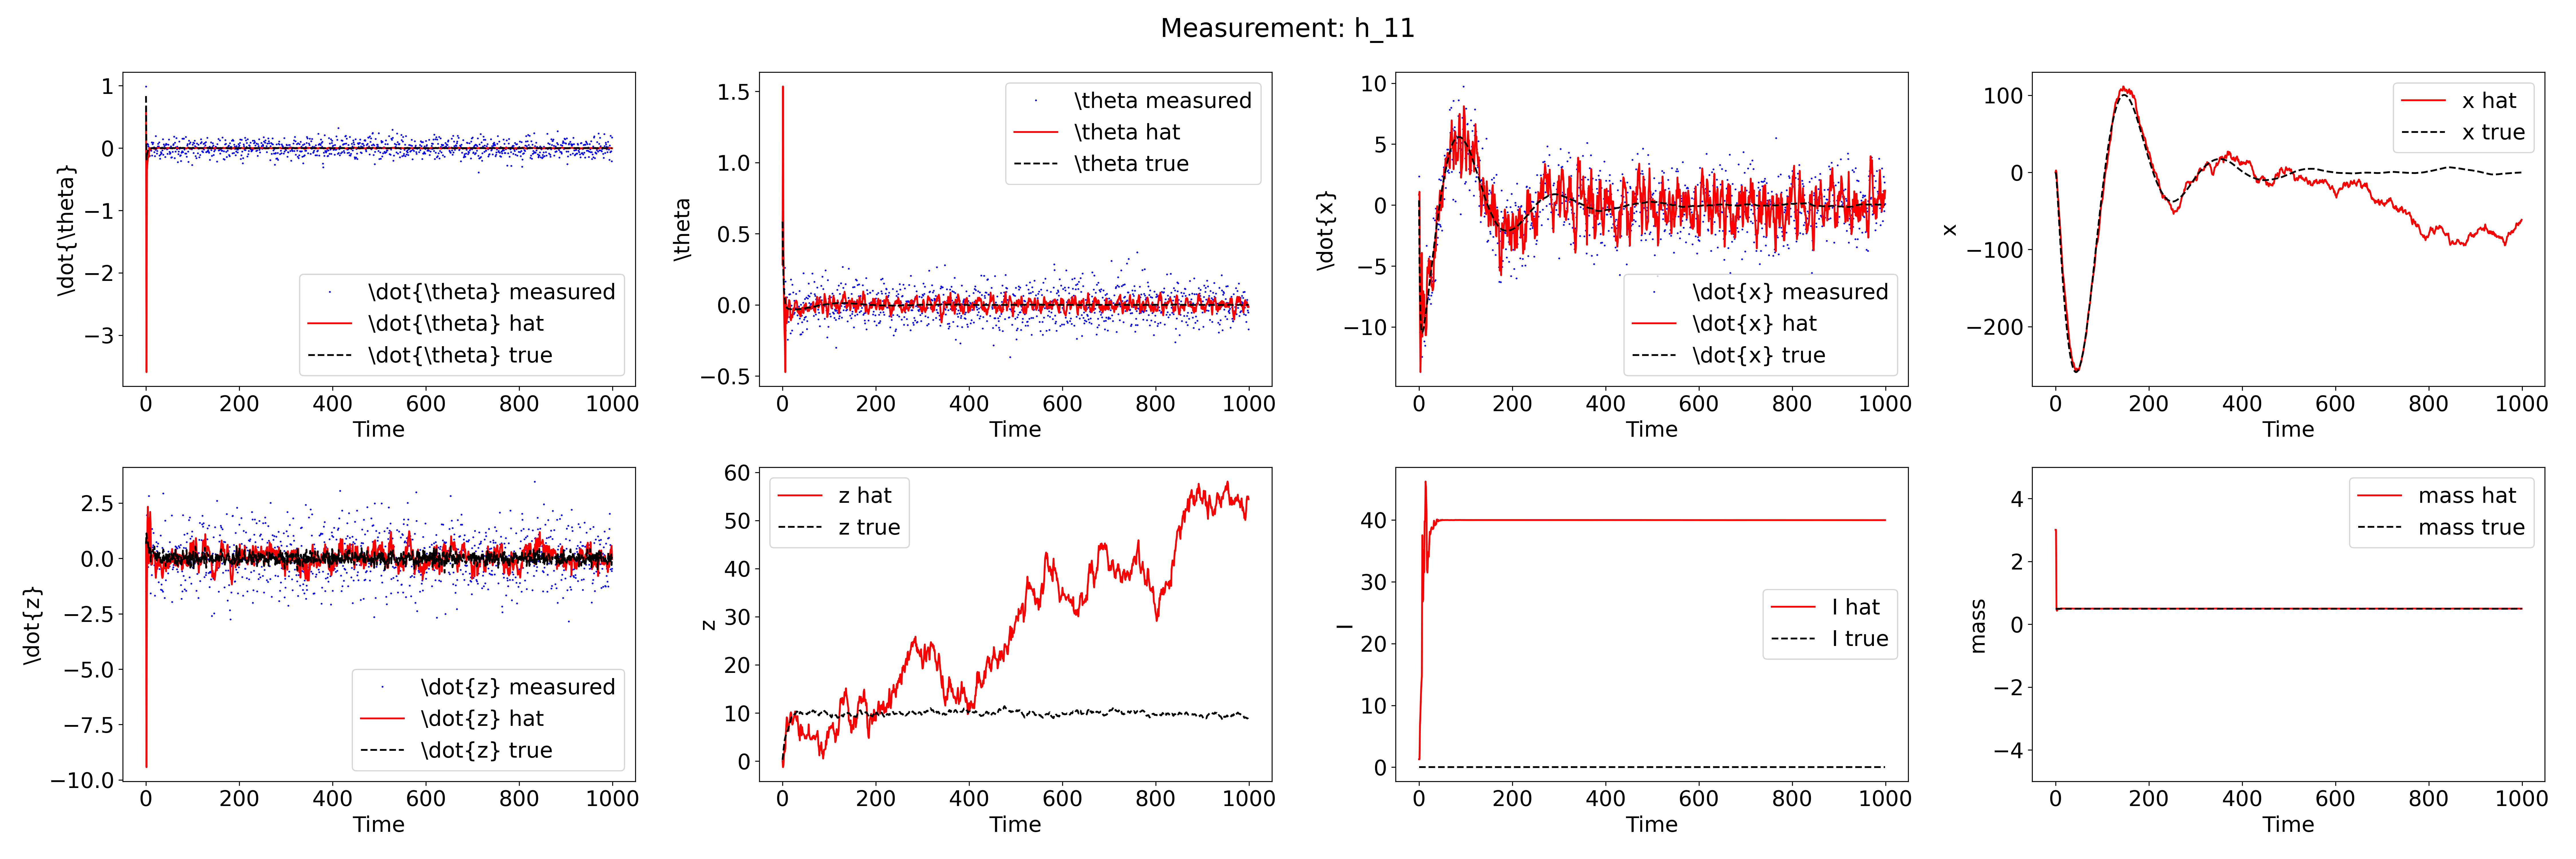
\includegraphics[width=15cm]{figures/ekf_with_noisy_sinusoidal_x_and_h11.png}
        \caption{State estimation with h11 measurement matrix}
        \label{fig:05c}
    \end{subfigure}
\end{figure}

Although the estimated parameter values are quite close to the true values, not all the states are estimated accurately. Estimation gets better with more direct measurements. But for some reason, the if the parameters are directly measured, the estimation gets worse. Further investigation is needed to understand the behavior of the system. To illustrate my point, here is the plot of the estimated states with a measurement matrix that directly measures all the real states. \ref{fig:05d}

\begin{figure}[H]
    \begin{subfigure}[t]{\textwidth}
        \centering
        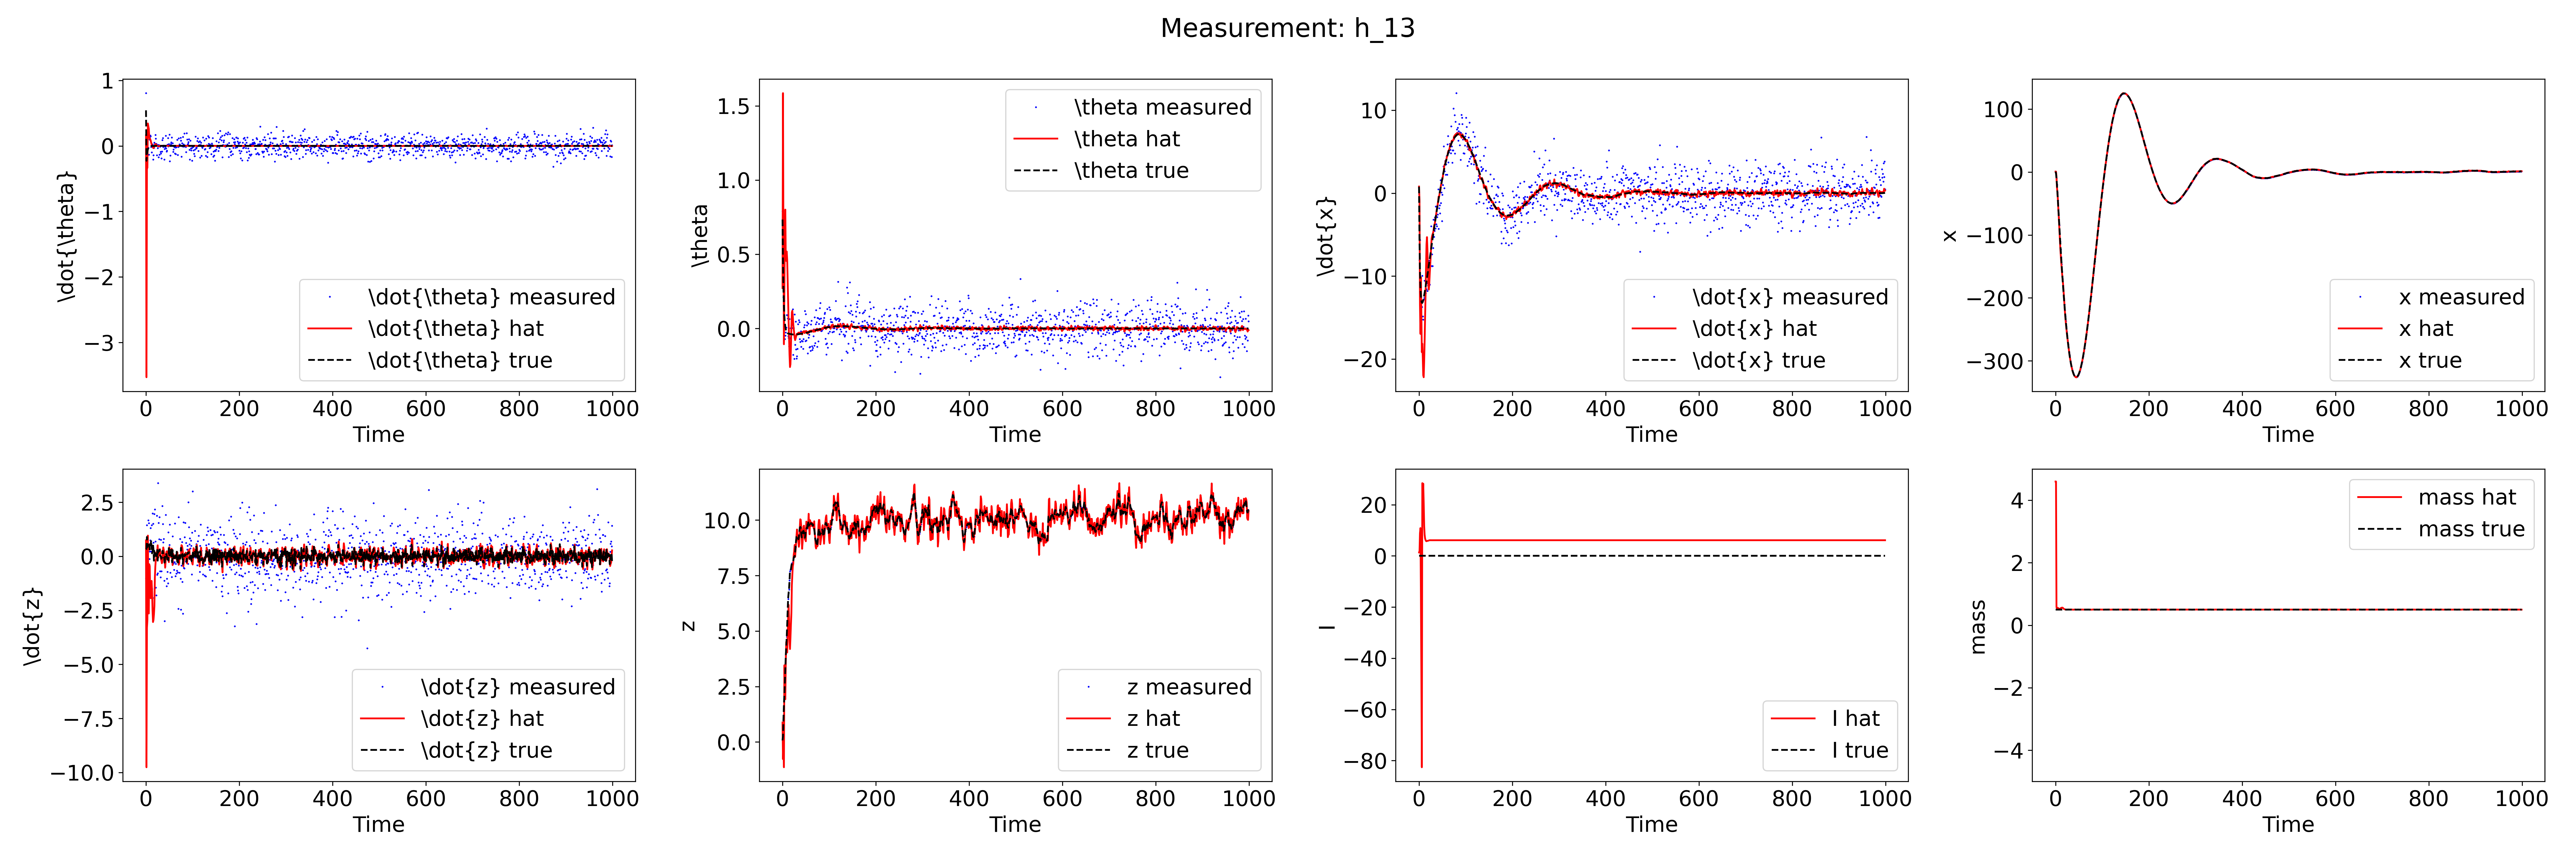
\includegraphics[width=15cm]{figures/ekf_with_noisy_sinusoidal_x_and_h13.png}
        \caption{State estimation with h13 measurement matrix}
        \label{fig:05d}
    \end{subfigure}
\end{figure}


\section*{Conclusion}
Observability is one of the most important aspects of a system. It is important to know if the measurements are enough to estimate the states of the system or not. In this paper, I have used different tools to estimate the observability of the system. The results although not conclusive yet, show the importance of observability analysis for state estimation. The parameter estimation is close to the true values but the state estimation is not as accurate all the time. Taking a look into their discrete dynamics might give a better understanding of the system.

\pagebreak
\bibliographystyle{plain}
\bibliography{phase0}


\section*{Suplementary Material}
\subsection*{G matrix and O matrix:}

\begin{align*}
    G &= \left[\begin{matrix}0\\- g\\\theta\\x\\\beta_{3}\\\dot{\theta}\\\beta_{1}\\\beta_{2}\\z\\\dot{x}\\\dot{z}\end{matrix}\right], 
    \left[\begin{matrix}0\\- g\\\theta\\x\\\beta_{3}\\\dot{\theta}\\\beta_{1}\\\beta_{2}\\z\\\dot{x}\\\dot{z}\end{matrix}\right], 
    \left[\begin{matrix}0\\\theta\\x\\\dot{x}\\\dot{\theta}\\\beta_{1}\\\beta_{2}\end{matrix}\right], 
    \left[\begin{matrix}0\\\beta_{1} x z\\\theta x z\\\beta_{2} \theta z + \beta_{3} \theta x\\\dot{\theta} x z + \dot{x} \theta z + \dot{z} \theta x\\\dot{\theta} \left(\dot{x} z + \dot{z} x\right) + \dot{x} \left(\dot{\theta} z + \dot{z} \theta\right) + \dot{z} \left(\dot{\theta} x + \dot{x} \theta\right) - g \theta x\end{matrix}\right],
    \left[\begin{matrix}0\\\dot{x} z + \dot{z} x\\x z\\\theta\\\beta_{2} z + \beta_{3} x\\\dot{\theta}\\2 \dot{x} \dot{z} - g x\\\beta_{1}\end{matrix}\right] \\
    &= ,\left[\begin{matrix}0\\- g\\\theta\\\beta_{3}\\\dot{\theta}\\\beta_{1}\\x + z\\z\\\beta_{2} + \beta_{3}\\\dot{x} + \dot{z}\\\dot{z}\end{matrix}\right],
    \left[\begin{matrix}0\\- g\\\beta_{2} + \beta_{3}\\\beta_{2}\\\theta + x\\\dot{\theta} + \dot{x}\\\dot{x} + \dot{z}\\\beta_{1}\\x + z\end{matrix}\right],
    \left[\begin{matrix}0\\- g\\\dot{\theta} + \dot{z}\\\beta_{3}\\\theta + x\\\beta_{1}\\x + z\\\beta_{2}\\\beta_{2} + \beta_{3}\\\dot{\theta} + \dot{x}\\\dot{x} + \dot{z}\\\theta + z\end{matrix}\right],
    \left[\begin{matrix}0\\- g\\\dot{\theta} x + \dot{x} \theta\\\dot{\theta} + \dot{z}\\\beta_{3}\\2 \dot{\theta} \dot{x}\\- \frac{\dot{x} z}{x^{2}} + \frac{\dot{z}}{x}\\\theta x\\\frac{z}{x}\\- \frac{\beta_{2} z}{x^{2}} + \frac{\beta_{3}}{x}\\\beta_{1}\\- \frac{\dot{x} \dot{z}}{x^{2}} + \dot{x} \left(\frac{2 \dot{x} z}{x^{3}} - \frac{\dot{z}}{x^{2}}\right) - \frac{g}{x}\\\beta_{1} x\\\theta + z\\\beta_{2} \theta\end{matrix}\right],
    \left[\begin{matrix}0\\- \frac{\dot{x} \dot{z}}{x^{2}} + \dot{x} \left(\frac{2 \dot{x} z}{x^{3}} - \frac{\dot{z}}{x^{2}}\right) - \frac{g}{x}\\\dot{\theta} x + \dot{x} \theta\\\beta_{1} x\\2 \dot{\theta} \dot{x}\\\beta_{2} \theta\\- \frac{\dot{x} z}{x^{2}} + \frac{\dot{z}}{x}\\\theta x\\\frac{z}{x}\\- \frac{\beta_{2} z}{x^{2}} + \frac{\beta_{3}}{x}\end{matrix}\right] \\
    &= \left[\begin{matrix}0\\\dot{z}\\- g\\\beta_{2}\\\beta_{1}\\\dot{x}\\\dot{\theta}\end{matrix}\right], 
    \left[\begin{matrix}0\\\dot{z}\\- g\\\beta_{2}\\\beta_{1}\\\dot{x}\\\dot{\theta}\\\theta\end{matrix}\right],
    \left[\begin{matrix}0\\\dot{z}\\\frac{\dot{\theta}}{\theta}\\\frac{\beta_{1}}{\theta}\\\dot{\theta}\\\log{\left(\theta \right)}\\- g\\\beta_{2}\\- \frac{\dot{\theta}^{2}}{\theta^{2}}\\\beta_{1}\\\dot{x}\end{matrix}\right]
\end{align*}

\begin{align*}
    O &= 
    \left[\begin{matrix}0 & 0 & 0 & 0 & 0 & 0 & 0 & 0\\0 & 0 & 0 & 0 & 1 & 0 & 0 & 0\\1 & 0 & 0 & 0 & 0 & 0 & 0 & 0\\0 & 0 & 0 & 0 & 0 & 1 & 0 & 0\\0 & 1 & 0 & 0 & 0 & 0 & 0 & 0\\0 & 0 & 0 & 0 & 0 & 0 & 0 & 0\\0 & 0 & 0 & 0 & 0 & 0 & 0 & 1\\0 & 0 & 0 & 1 & 0 & 0 & 0 & 0\\0 & 0 & 1 & 0 & 0 & 0 & 0 & 0\\0 & 0 & 0 & 0 & 0 & 0 & 1 & 0\end{matrix}\right], 
    \left[\begin{matrix}0 & 0 & 0 & 0 & 0 & 0 & 0 & 0\\0 & 0 & 0 & 0 & 1 & 0 & 0 & 0\\1 & 0 & 0 & 0 & 0 & 0 & 0 & 0\\0 & 0 & 0 & 0 & 0 & 1 & 0 & 0\\0 & 1 & 0 & 0 & 0 & 0 & 0 & 0\\0 & 0 & 0 & 0 & 0 & 0 & 0 & 0\\0 & 0 & 0 & 0 & 0 & 0 & 0 & 1\\0 & 0 & 0 & 1 & 0 & 0 & 0 & 0\\0 & 0 & 1 & 0 & 0 & 0 & 0 & 0\\0 & 0 & 0 & 0 & 0 & 0 & 1 & 0\end{matrix}\right], 
    \left[\begin{matrix}0 & 0 & 0 & 0 & 0 & 0 & 0 & 0\\0 & 0 & 0 & 0 & 0 & 0 & 0 & 1\\0 & 0 & 0 & 1 & 0 & 0 & 0 & 0\\0 & 0 & 1 & 0 & 0 & 0 & 0 & 0\\0 & 0 & 0 & 0 & 0 & 0 & 1 & 0\\1 & 0 & 0 & 0 & 0 & 0 & 0 & 0\\0 & 1 & 0 & 0 & 0 & 0 & 0 & 0\end{matrix}\right], \\
    &=
    \left[\begin{matrix}0 & 0 & 0 & 0 & 0 & 0 & 0 & 0\\0 & 0 & 0 & \beta_{1} z & 0 & \beta_{1} x & x z & 0\\x z & \dot{x} z + \dot{z} x & \theta z & \dot{\theta} z + \dot{z} \theta & \theta x & \dot{\theta} x + \dot{x} \theta & 0 & 0\\2 \dot{x} z + 2 \dot{z} x & 2 \dot{x} \dot{z} - g x & 2 \dot{\theta} z + 2 \dot{z} \theta & 2 \dot{\theta} \dot{z} - \theta g & 2 \dot{\theta} x + 2 \dot{x} \theta & 2 \dot{\theta} \dot{x} & 0 & 0\\0 & x z & 0 & \theta z & 0 & \theta x & 0 & 0\\0 & \beta_{2} x + \beta_{2} z & 0 & \beta_{2} \theta & 0 & \beta_{2} \theta & 0 & \theta x + \theta z\end{matrix}\right], \\
    &= 
    \left[\begin{matrix}0 & 0 & 0 & 0 & 0 & 0 & 0 & 0\\0 & 0 & 0 & z & 0 & x & 0 & 0\\0 & 0 & 2 \dot{z} & - g & 2 \dot{x} & 0 & 0 & 0\\0 & 0 & z & \dot{z} & x & \dot{x} & 0 & 0\\0 & 0 & 0 & 0 & 0 & 0 & 1 & 0\\1 & 0 & 0 & 0 & 0 & 0 & 0 & 0\\0 & 0 & 0 & \beta_{2} & 0 & \beta_{2} & 0 & x + z\\0 & 1 & 0 & 0 & 0 & 0 & 0 & 0\end{matrix}\right],
    \left[\begin{matrix}0 & 0 & 0 & 0 & 0 & 0 & 0 & 0\\0 & 0 & 0 & 1 & 0 & 1 & 0 & 0\\0 & 0 & 1 & 0 & 1 & 0 & 0 & 0\\0 & 0 & 0 & 0 & 1 & 0 & 0 & 0\\1 & 0 & 0 & 0 & 0 & 0 & 0 & 0\\0 & 0 & 0 & 0 & 0 & 1 & 0 & 0\\0 & 1 & 0 & 0 & 0 & 0 & 0 & 0\\0 & 0 & 0 & 0 & 0 & 0 & 0 & 0\\0 & 0 & 0 & 0 & 0 & 0 & 0 & 2\\0 & 0 & 0 & 0 & 0 & 0 & 0 & 1\\0 & 0 & 0 & 0 & 0 & 0 & 1 & 0\end{matrix}\right], \\
    &=
    \left[\begin{matrix}0 & 0 & 0 & 0 & 0 & 0 & 0 & 0\\0 & 0 & 0 & 1 & 0 & 1 & 0 & 0\\0 & 0 & 1 & 0 & 1 & 0 & 0 & 0\\0 & 0 & 0 & 0 & 0 & 0 & 0 & 0\\0 & 0 & 0 & 0 & 0 & 0 & 0 & 2\\0 & 0 & 0 & 0 & 0 & 0 & 0 & 1\\1 & 0 & 1 & 0 & 0 & 0 & 0 & 0\\0 & 0 & 0 & 0 & 0 & 0 & 1 & 0\\0 & 1 & 0 & 1 & 0 & 0 & 0 & 0\end{matrix}\right],
    \left[\begin{matrix}0 & 0 & 0 & 0 & 0 & 0 & 0 & 0\\0 & 0 & 0 & 1 & 0 & 1 & 0 & 0\\0 & 0 & 1 & 0 & 1 & 0 & 0 & 0\\1 & 0 & 1 & 0 & 0 & 0 & 0 & 0\\0 & 1 & 0 & 1 & 0 & 0 & 0 & 0\\1 & 0 & 0 & 0 & 1 & 0 & 0 & 0\\0 & 0 & 0 & 0 & 0 & 0 & 0 & 0\\0 & 0 & 0 & 0 & 0 & 0 & 0 & 2\\0 & 1 & 0 & 0 & 0 & 1 & 0 & 0\\0 & 0 & 0 & 0 & 0 & 0 & 0 & 1\\0 & 0 & 0 & 0 & 0 & 0 & 1 & 0\end{matrix}\right]
\end{align*}

\begin{align*}
    O &=
    \left[\begin{matrix}0 & 0 & 0 & 0 & 0 & 0 & 0 & 0\\0 & 0 & \frac{4 \dot{x} z}{x^{3}} - \frac{2 \dot{z}}{x^{2}} & \frac{2 \dot{x} \dot{z}}{x^{3}} + \dot{x} \left(- \frac{6 \dot{x} z}{x^{4}} + \frac{2 \dot{z}}{x^{3}}\right) + \frac{g}{x^{2}} & - \frac{2 \dot{x}}{x^{2}} & \frac{2 \dot{x}^{2}}{x^{3}} & 0 & 0\\0 & \beta_{2} & 0 & 0 & 0 & 0 & 0 & \theta\\0 & 0 & 0 & - \frac{z}{x^{2}} & 0 & \frac{1}{x} & 0 & 0\\1 & 0 & 0 & 0 & 1 & 0 & 0 & 0\\0 & 0 & 0 & - \frac{\beta_{2}}{x^{2}} + \frac{2 \beta_{2} z}{x^{3}} & 0 & - \frac{\beta_{2}}{x^{2}} & 0 & \frac{1}{x} - \frac{z}{x^{2}}\\0 & 0 & - \frac{z}{x^{2}} & \frac{2 \dot{x} z}{x^{3}} - \frac{\dot{z}}{x^{2}} & \frac{1}{x} & - \frac{\dot{x}}{x^{2}} & 0 & 0\\0 & 0 & 0 & \beta_{1} & 0 & 0 & x & 0\\0 & 0 & 0 & 0 & 0 & 0 & 0 & 0\\0 & 1 & 0 & 0 & 0 & 1 & 0 & 0\\0 & 0 & 0 & 0 & 0 & 0 & 0 & 1\\0 & 0 & 0 & 0 & 0 & 0 & 1 & 0\\x & \dot{x} & \theta & \dot{\theta} & 0 & 0 & 0 & 0\\0 & x & 0 & \theta & 0 & 0 & 0 & 0\\2 \dot{x} & 0 & 2 \dot{\theta} & 0 & 0 & 0 & 0 & 0\end{matrix}\right], \\
    &=
    \left[\begin{matrix}0 & 0 & 0 & 0 & 0 & 0 & 0 & 0\\0 & 0 & 0 & - \frac{\beta_{2}}{x^{2}} + \frac{2 \beta_{2} z}{x^{3}} & 0 & - \frac{\beta_{2}}{x^{2}} & 0 & \frac{1}{x} - \frac{z}{x^{2}}\\0 & 0 & - \frac{z}{x^{2}} & \frac{2 \dot{x} z}{x^{3}} - \frac{\dot{z}}{x^{2}} & \frac{1}{x} & - \frac{\dot{x}}{x^{2}} & 0 & 0\\0 & 0 & 0 & \beta_{1} & 0 & 0 & x & 0\\0 & 0 & \frac{4 \dot{x} z}{x^{3}} - \frac{2 \dot{z}}{x^{2}} & \frac{2 \dot{x} \dot{z}}{x^{3}} + \dot{x} \left(- \frac{6 \dot{x} z}{x^{4}} + \frac{2 \dot{z}}{x^{3}}\right) + \frac{g}{x^{2}} & - \frac{2 \dot{x}}{x^{2}} & \frac{2 \dot{x}^{2}}{x^{3}} & 0 & 0\\0 & \beta_{2} & 0 & 0 & 0 & 0 & 0 & \theta\\x & \dot{x} & \theta & \dot{\theta} & 0 & 0 & 0 & 0\\0 & x & 0 & \theta & 0 & 0 & 0 & 0\\0 & 0 & 0 & - \frac{z}{x^{2}} & 0 & \frac{1}{x} & 0 & 0\\2 \dot{x} & 0 & 2 \dot{\theta} & 0 & 0 & 0 & 0 & 0\end{matrix}\right], \\
    &=
    \left[\begin{matrix}0 & 0 & 0 & 0 & 0 & 0 & 0 & 0\\0 & 0 & 0 & 0 & 1 & 0 & 0 & 0\\0 & 0 & 0 & 0 & 0 & 0 & 0 & 0\\0 & 0 & 0 & 0 & 0 & 0 & 0 & 1\\0 & 0 & 0 & 0 & 0 & 0 & 1 & 0\\0 & 0 & 1 & 0 & 0 & 0 & 0 & 0\\1 & 0 & 0 & 0 & 0 & 0 & 0 & 0\end{matrix}\right], 
    \left[\begin{matrix}0 & 0 & 0 & 0 & 0 & 0 & 0 & 0\\0 & 0 & 0 & 0 & 1 & 0 & 0 & 0\\0 & 0 & 0 & 0 & 0 & 0 & 0 & 0\\0 & 0 & 0 & 0 & 0 & 0 & 0 & 1\\0 & 0 & 0 & 0 & 0 & 0 & 1 & 0\\0 & 0 & 1 & 0 & 0 & 0 & 0 & 0\\1 & 0 & 0 & 0 & 0 & 0 & 0 & 0\\0 & 1 & 0 & 0 & 0 & 0 & 0 & 0\end{matrix}\right], \\
    &=
    \left[\begin{matrix}0 & 0 & 0 & 0 & 0 & 0 & 0 & 0\\0 & 0 & 0 & 0 & 1 & 0 & 0 & 0\\\frac{1}{\theta} & - \frac{\dot{\theta}}{\theta^{2}} & 0 & 0 & 0 & 0 & 0 & 0\\0 & - \frac{\beta_{1}}{\theta^{2}} & 0 & 0 & 0 & 0 & \frac{1}{\theta} & 0\\1 & 0 & 0 & 0 & 0 & 0 & 0 & 0\\0 & \frac{1}{\theta} & 0 & 0 & 0 & 0 & 0 & 0\\0 & 0 & 0 & 0 & 0 & 0 & 0 & 0\\0 & 0 & 0 & 0 & 0 & 0 & 0 & 1\\- \frac{2 \dot{\theta}}{\theta^{2}} & \frac{2 \dot{\theta}^{2}}{\theta^{3}} & 0 & 0 & 0 & 0 & 0 & 0\\0 & 0 & 0 & 0 & 0 & 0 & 1 & 0\\0 & 0 & 1 & 0 & 0 & 0 & 0 & 0\end{matrix}\right]
\end{align*}


\subsection*{Observability analysis:h0}
here, the measurement matrix is equal to the state matrix.
\begin{figure}[H]
    \centering
    \begin{subfigure}[t]{\textwidth}
        \centering
        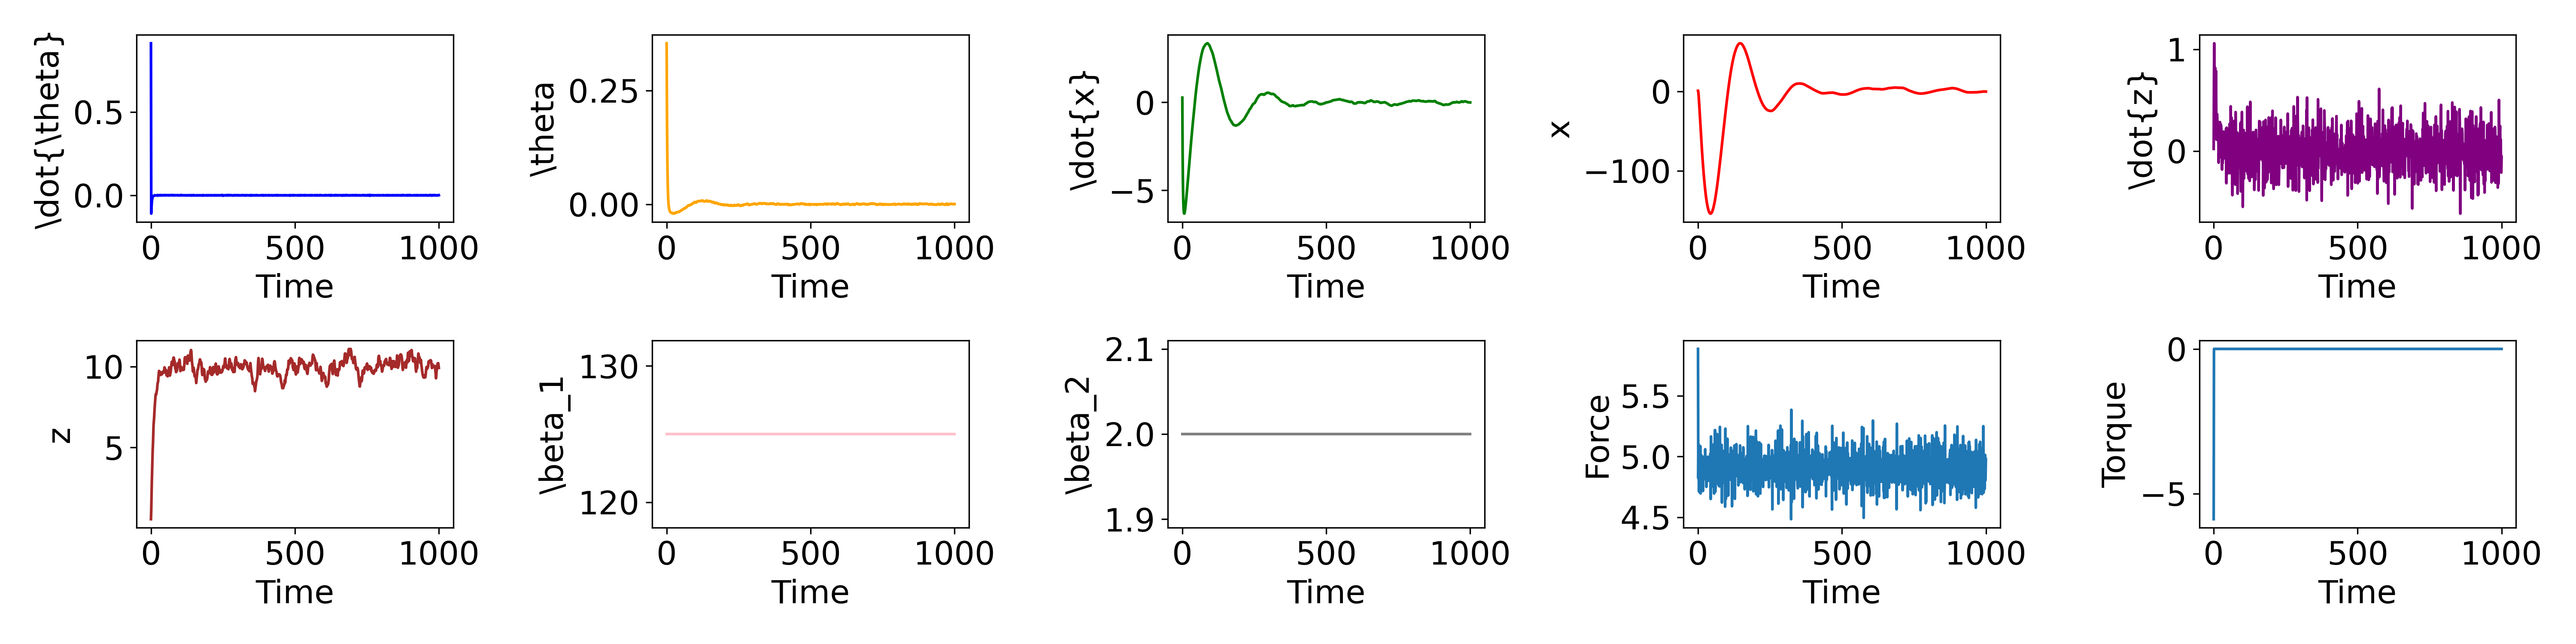
\includegraphics[width=15cm]{figures/states_with_noisy_sinusoidal_x_and_h0.png}
        \caption{State values with h0 measurement matrix}
        \label{supfig:01a}
    \end{subfigure}
    \\
    \begin{subfigure}[t]{\textwidth}
        \centering
        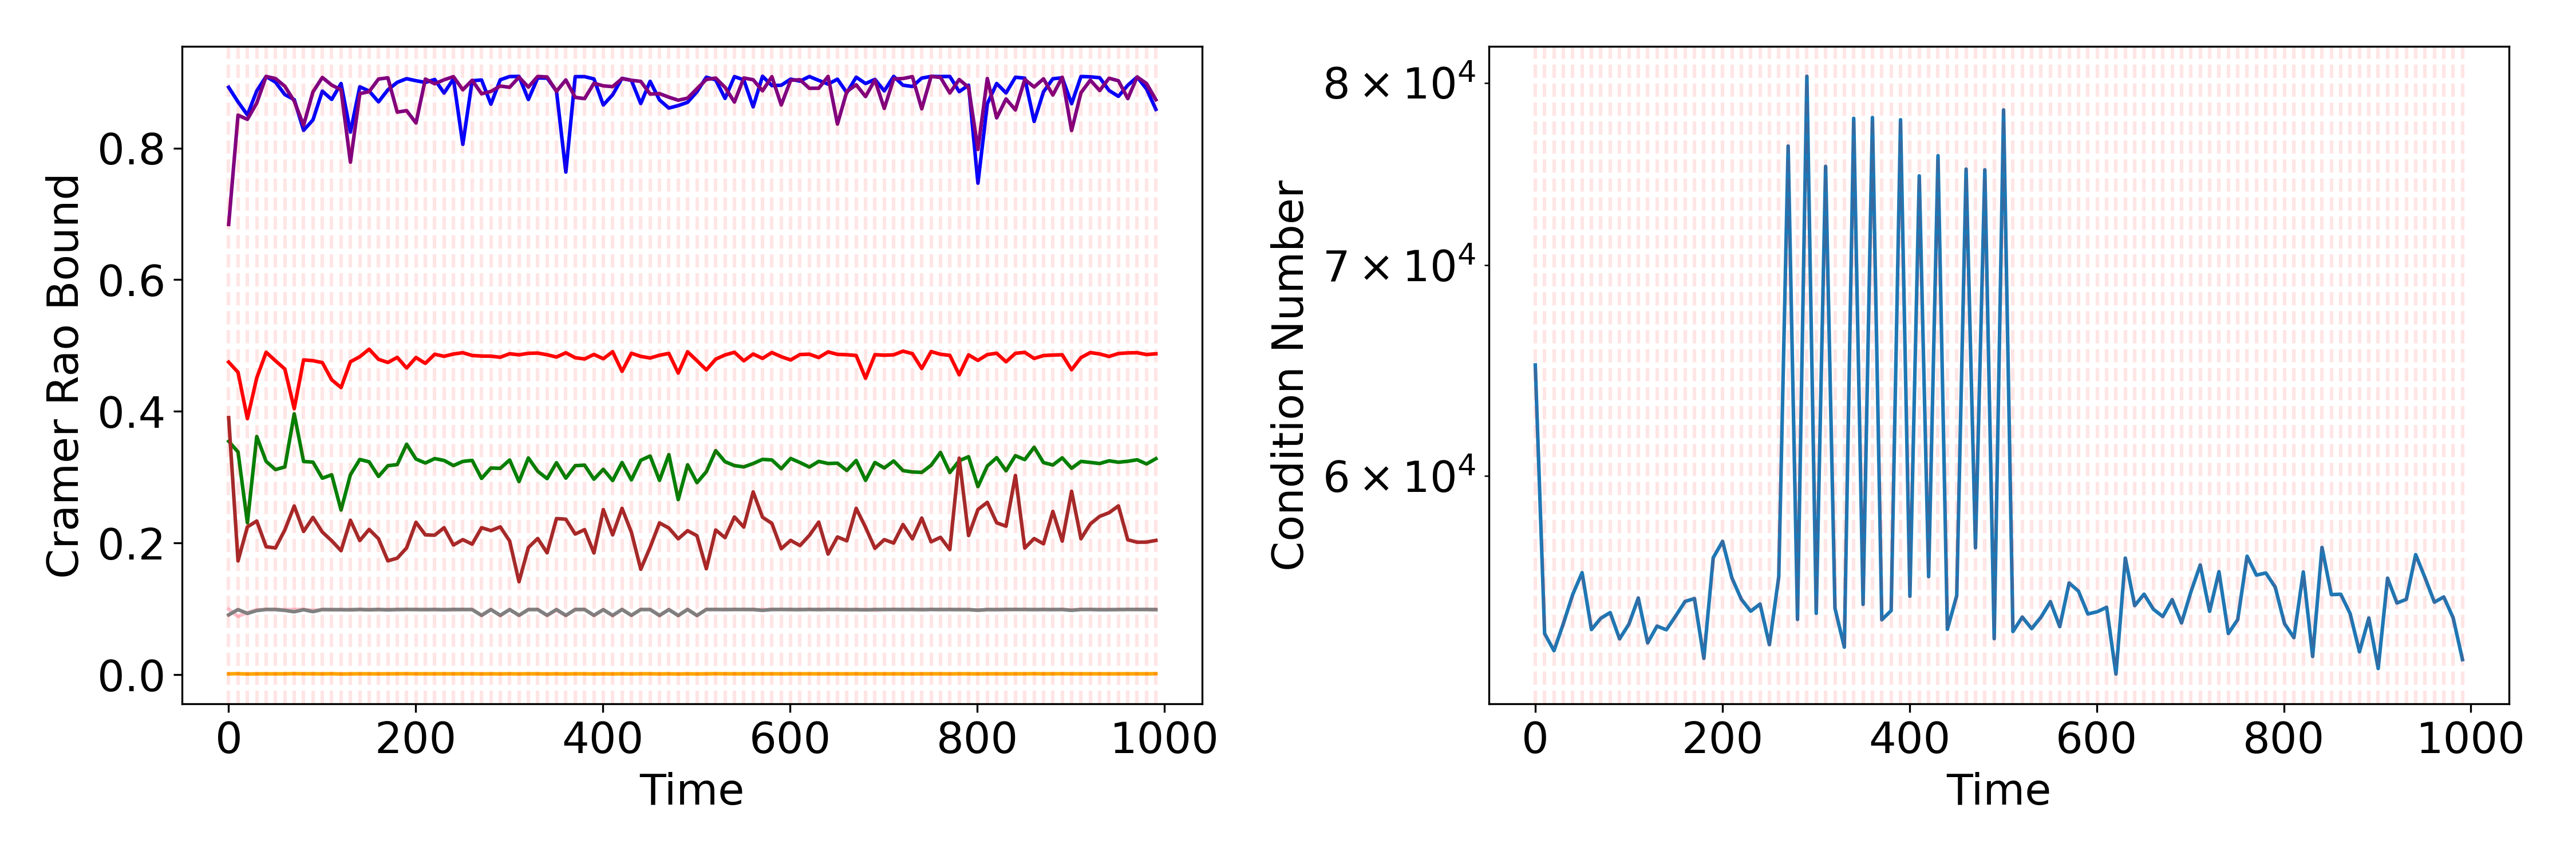
\includegraphics[width=15cm]{figures/crb_and_cn_with_noisy_sinusoidal_x_and_h0.png}
        \caption{Cramer Rao Lower Bound and Condition Number of the system with h0 measurement matrix}
        \label{supfig:01b}
    \end{subfigure}
    \\
    \begin{subfigure}[t]{\textwidth}
        \centering
        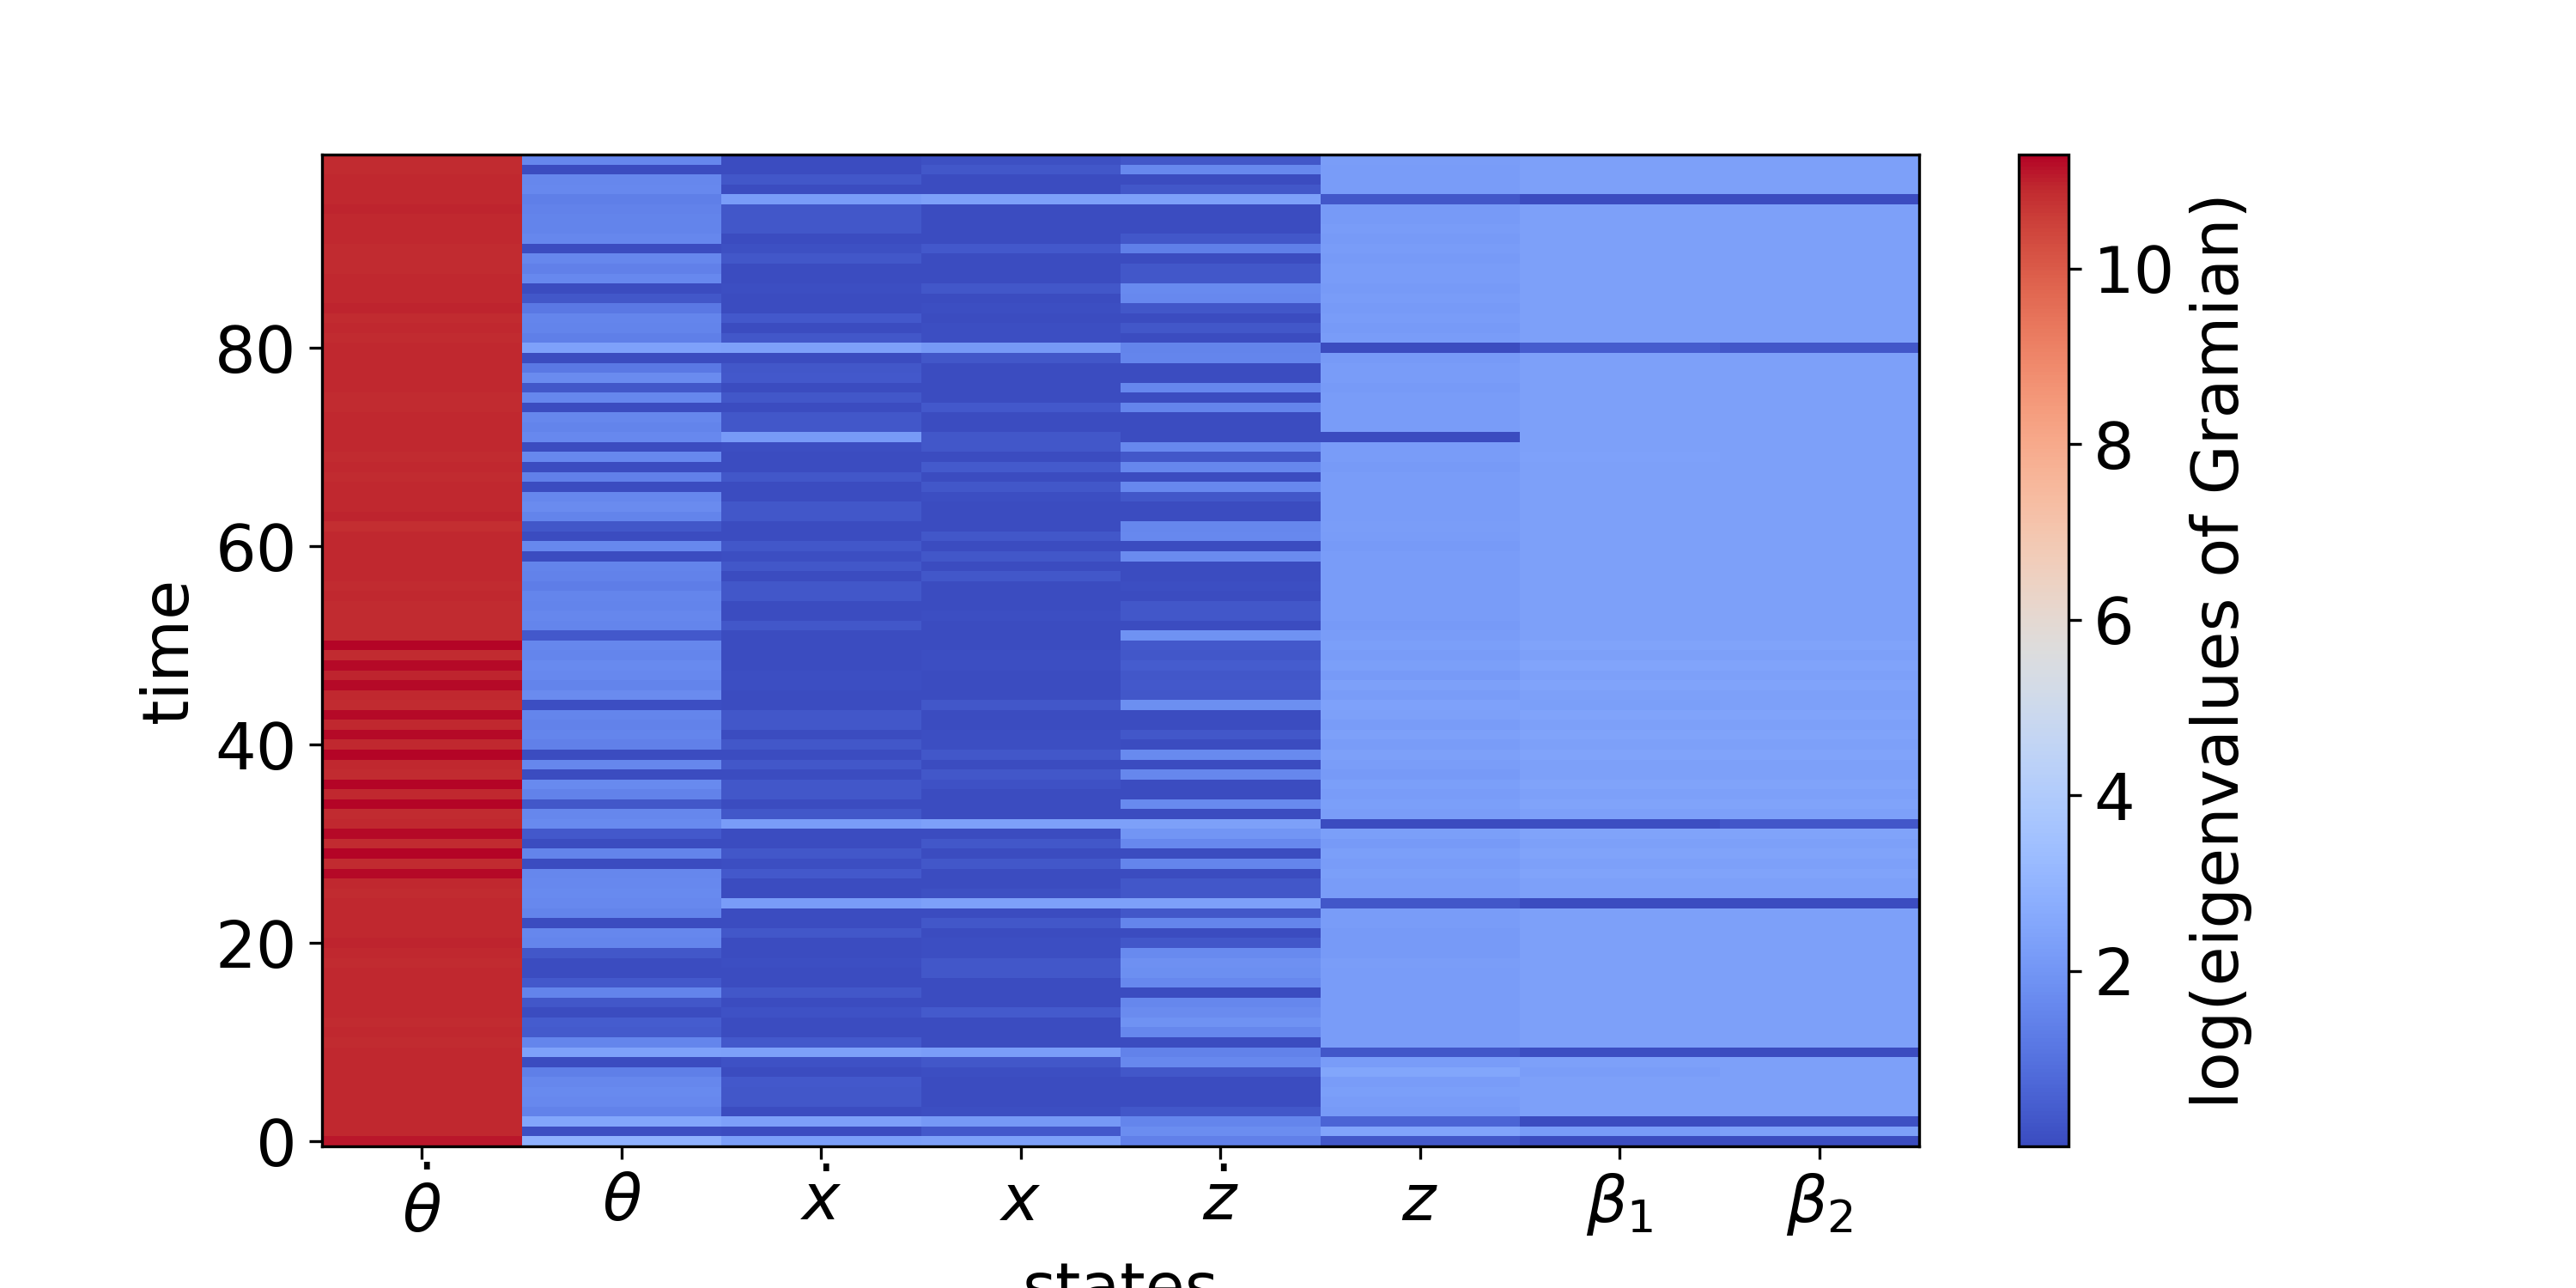
\includegraphics[width=15cm]{figures/gramian_eigenvalues_with_noisy_sinusoidal_x_and_h0.png}
        \caption{Eigenvalues of the Gramian matrix with time}
        \label{supfig:01c}
    \end{subfigure}
\end{figure}

\subsection*{Observability analysis:h9}
\begin{figure}[H]
    \centering
    \begin{subfigure}[t]{\textwidth}
        \centering
        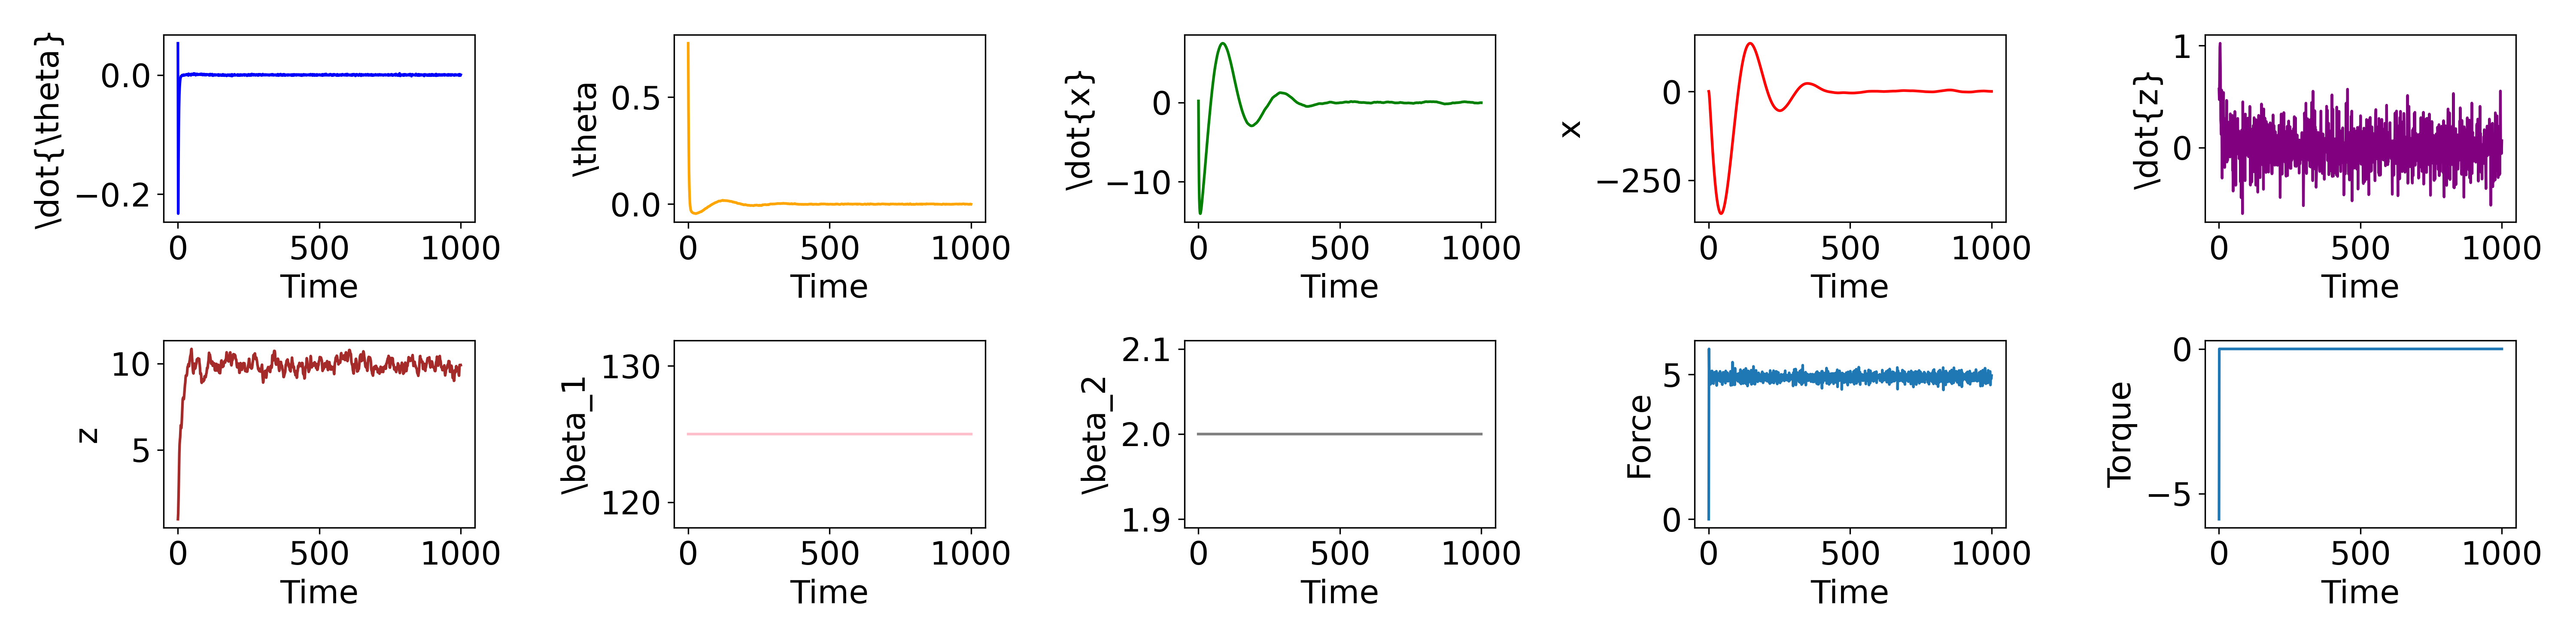
\includegraphics[width=15cm]{figures/states_with_noisy_sinusoidal_x_and_h9.png}
        \caption{State values with h9 measurement matrix}
        \label{supfig:09a}
    \end{subfigure}
    \\
    \begin{subfigure}[t]{\textwidth}
        \centering
        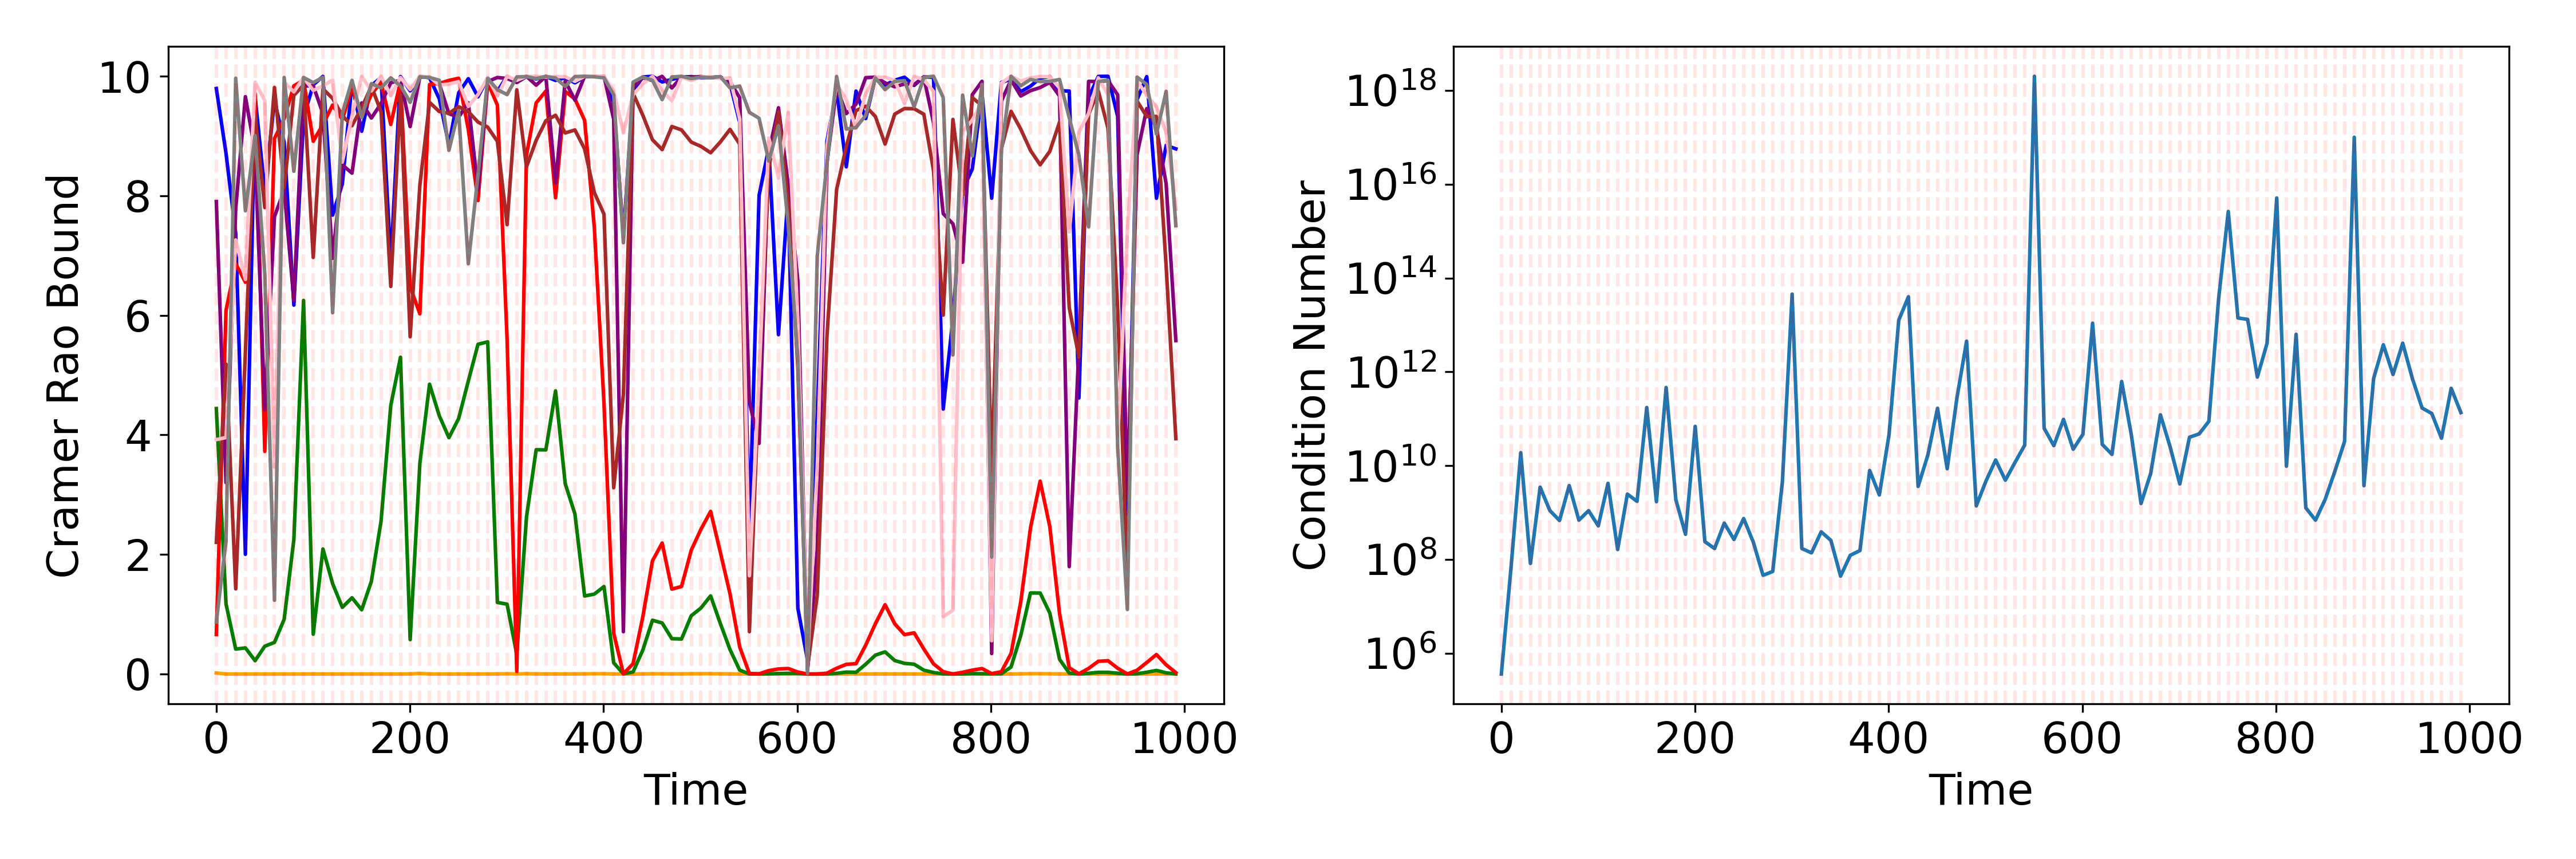
\includegraphics[width=15cm]{figures/crb_and_cn_with_noisy_sinusoidal_x_and_h9.png}
        \caption{Cramer Rao Lower Bound and Condition Number of the system with h9 measurement matrix}
        \label{supfig:09b}
    \end{subfigure}
    \\
    \begin{subfigure}[t]{\textwidth}
        \centering
        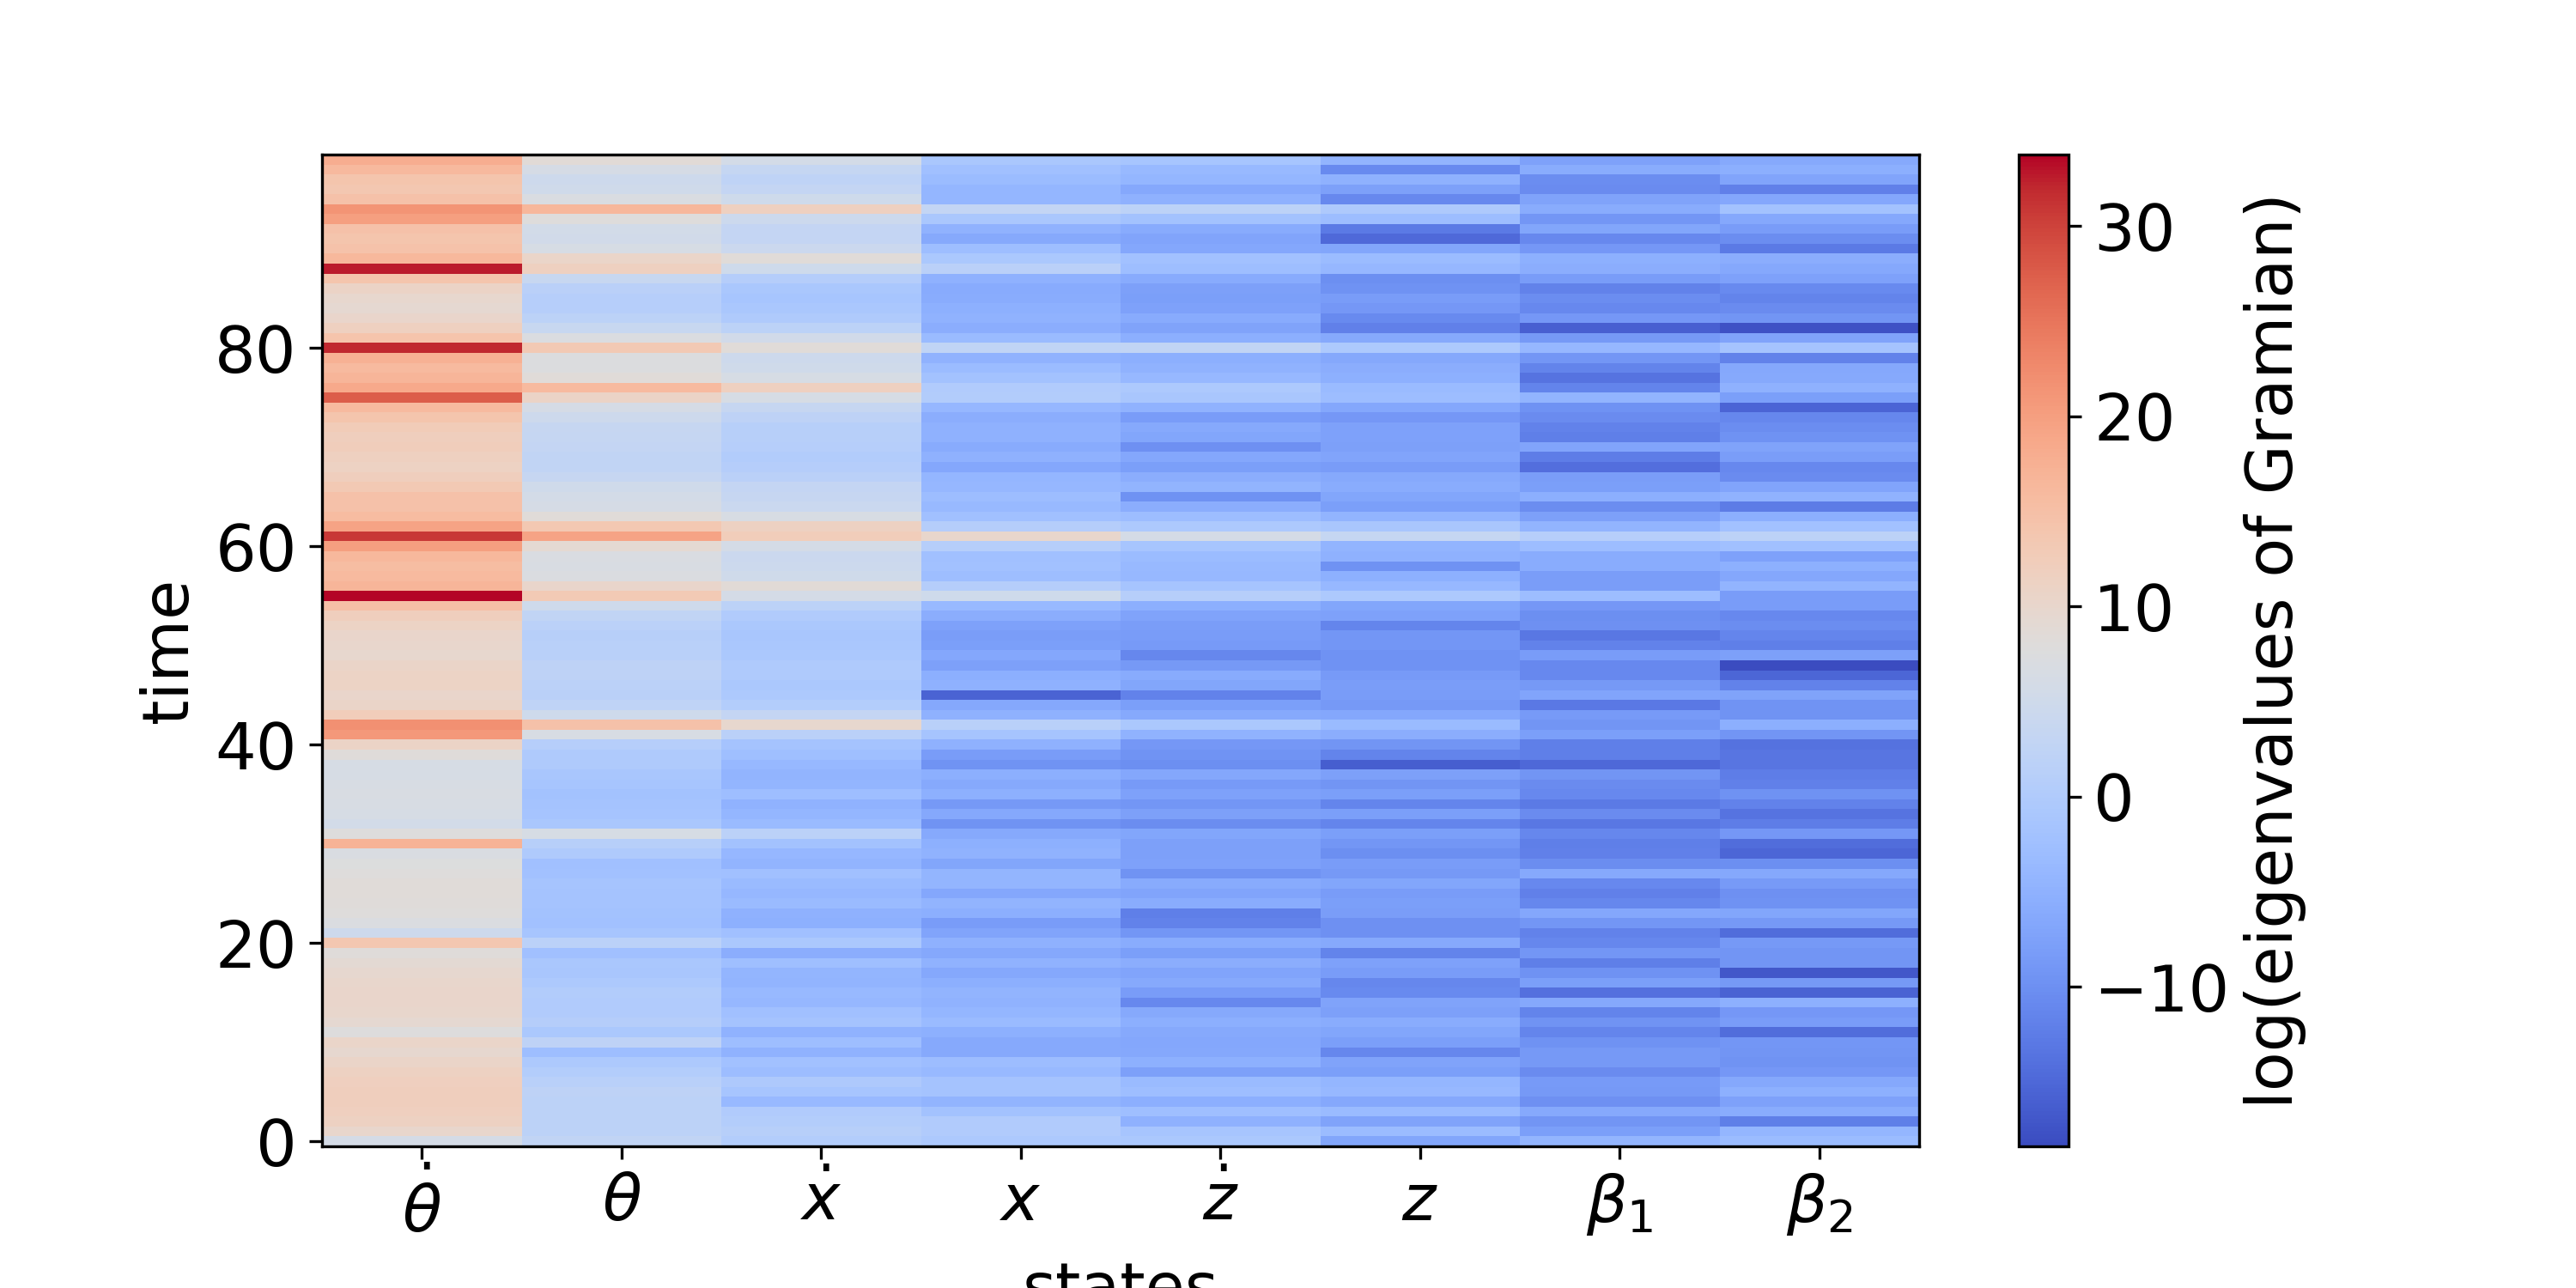
\includegraphics[width=15cm]{figures/gramian_eigenvalues_with_noisy_sinusoidal_x_and_h9.png}
        \caption{Eigenvalues of the Gramian matrix with time}
        \label{supfig:09c}
    \end{subfigure}
\end{figure}


\subsection*{Observability analysis:h13}
\begin{align*}
    h &= \left[\begin{matrix}\dot{\theta}\\\theta\\\dot{x}\\\dot{z}\\x\\z\end{matrix}\right]
\end{align*}

\begin{figure}[H]
    \centering
    \begin{subfigure}[t]{\textwidth}
        \centering
        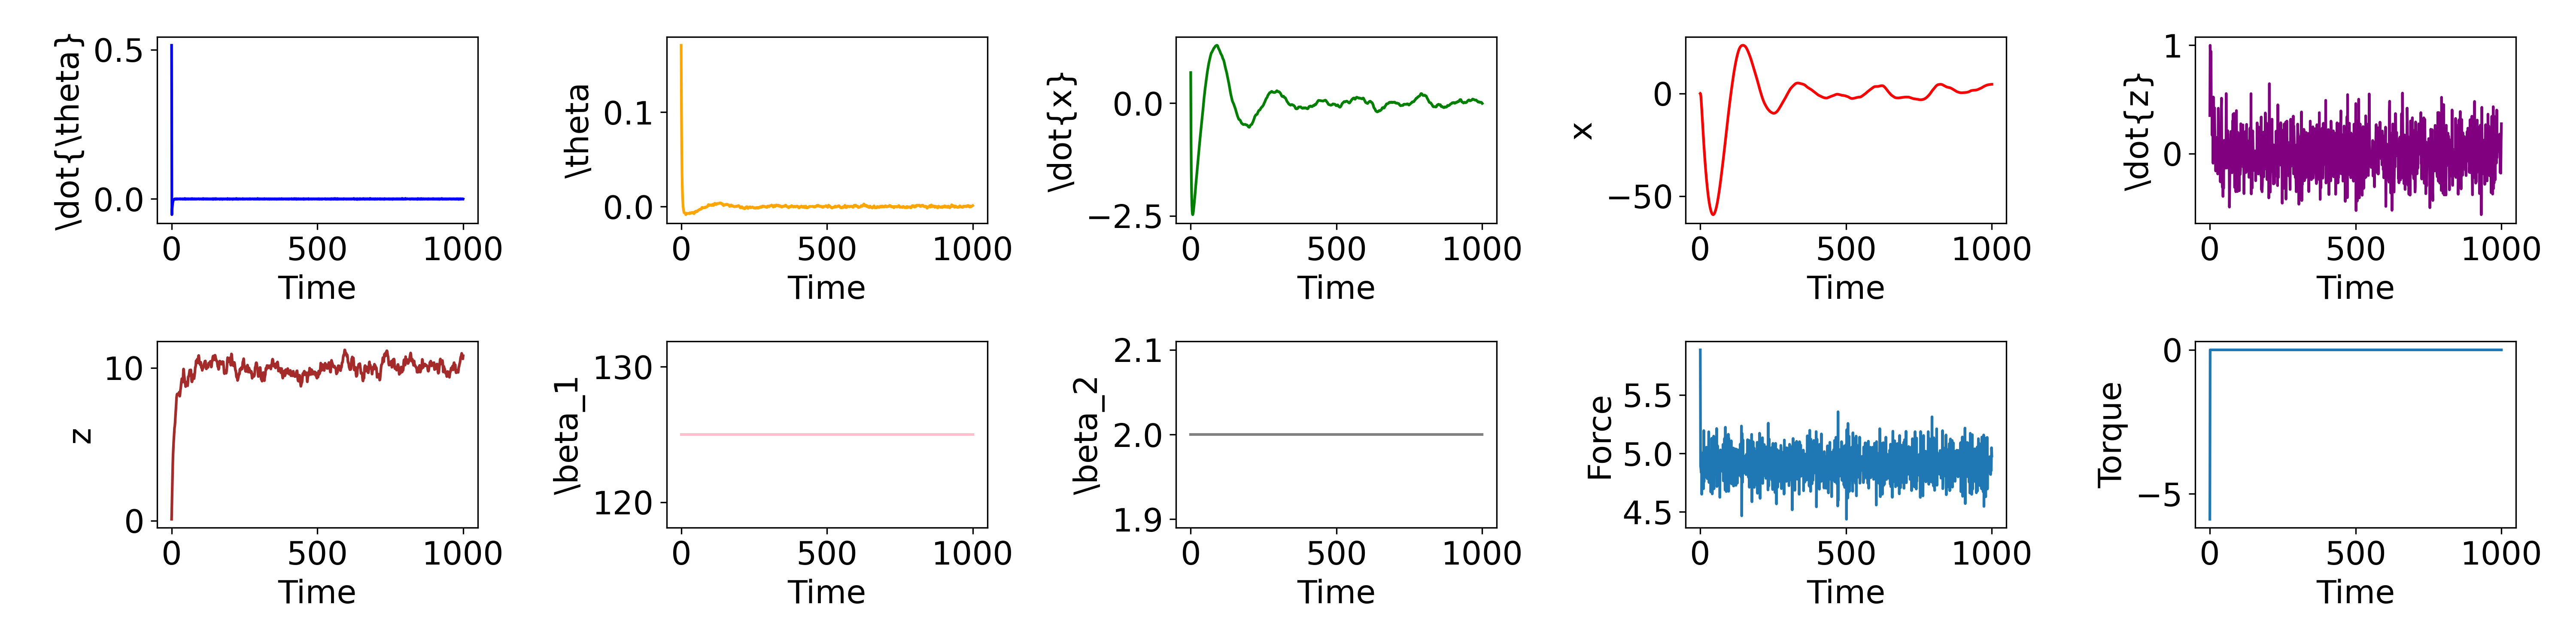
\includegraphics[width=15cm]{figures/states_with_noisy_sinusoidal_x_and_h13.png}
        \caption{State values with h13 measurement matrix}
        \label{supfig:09a}
    \end{subfigure}
    \\
    \begin{subfigure}[t]{\textwidth}
        \centering
        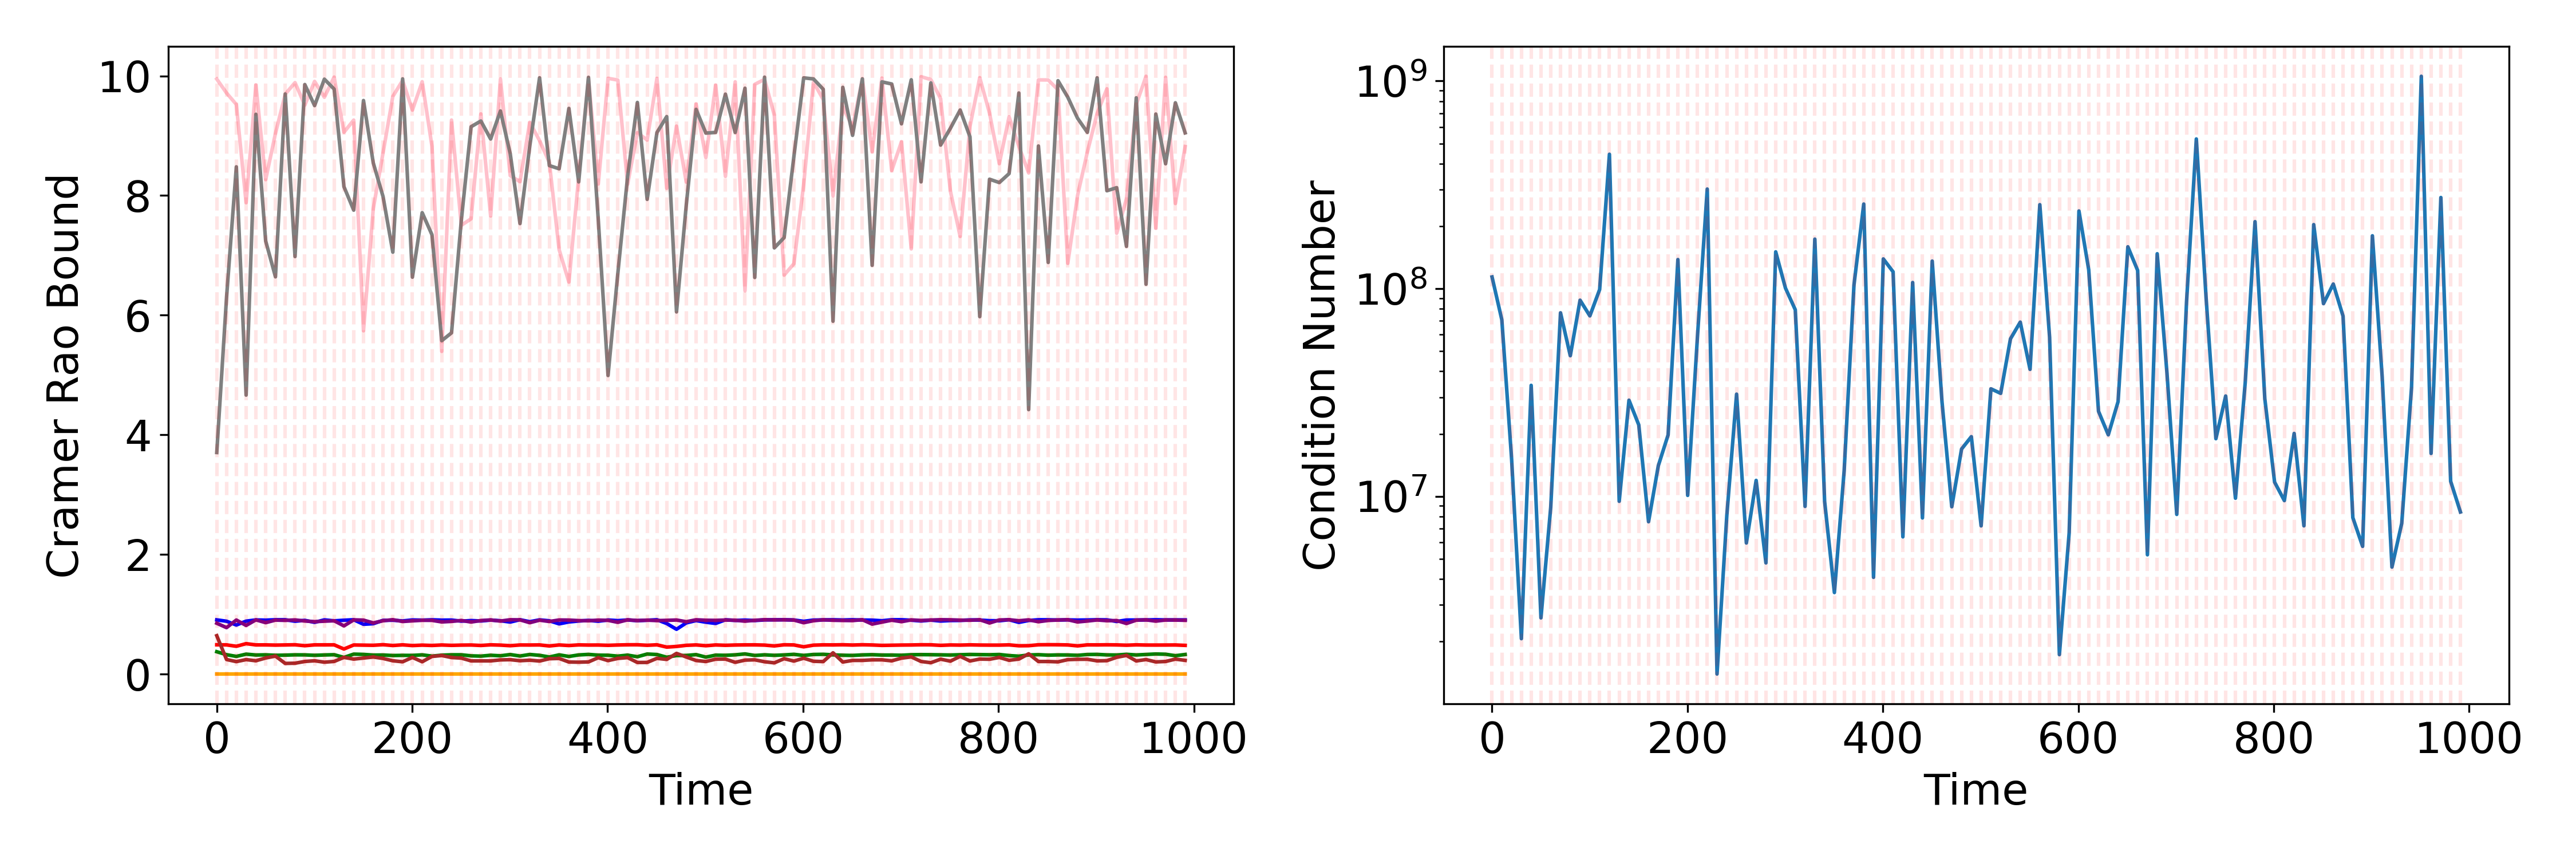
\includegraphics[width=15cm]{figures/crb_and_cn_with_noisy_sinusoidal_x_and_h13.png}
        \caption{Cramer Rao Lower Bound and Condition Number of the system with h13 measurement matrix}
        \label{supfig:09b}
    \end{subfigure}
    \\
    \begin{subfigure}[t]{\textwidth}
        \centering
        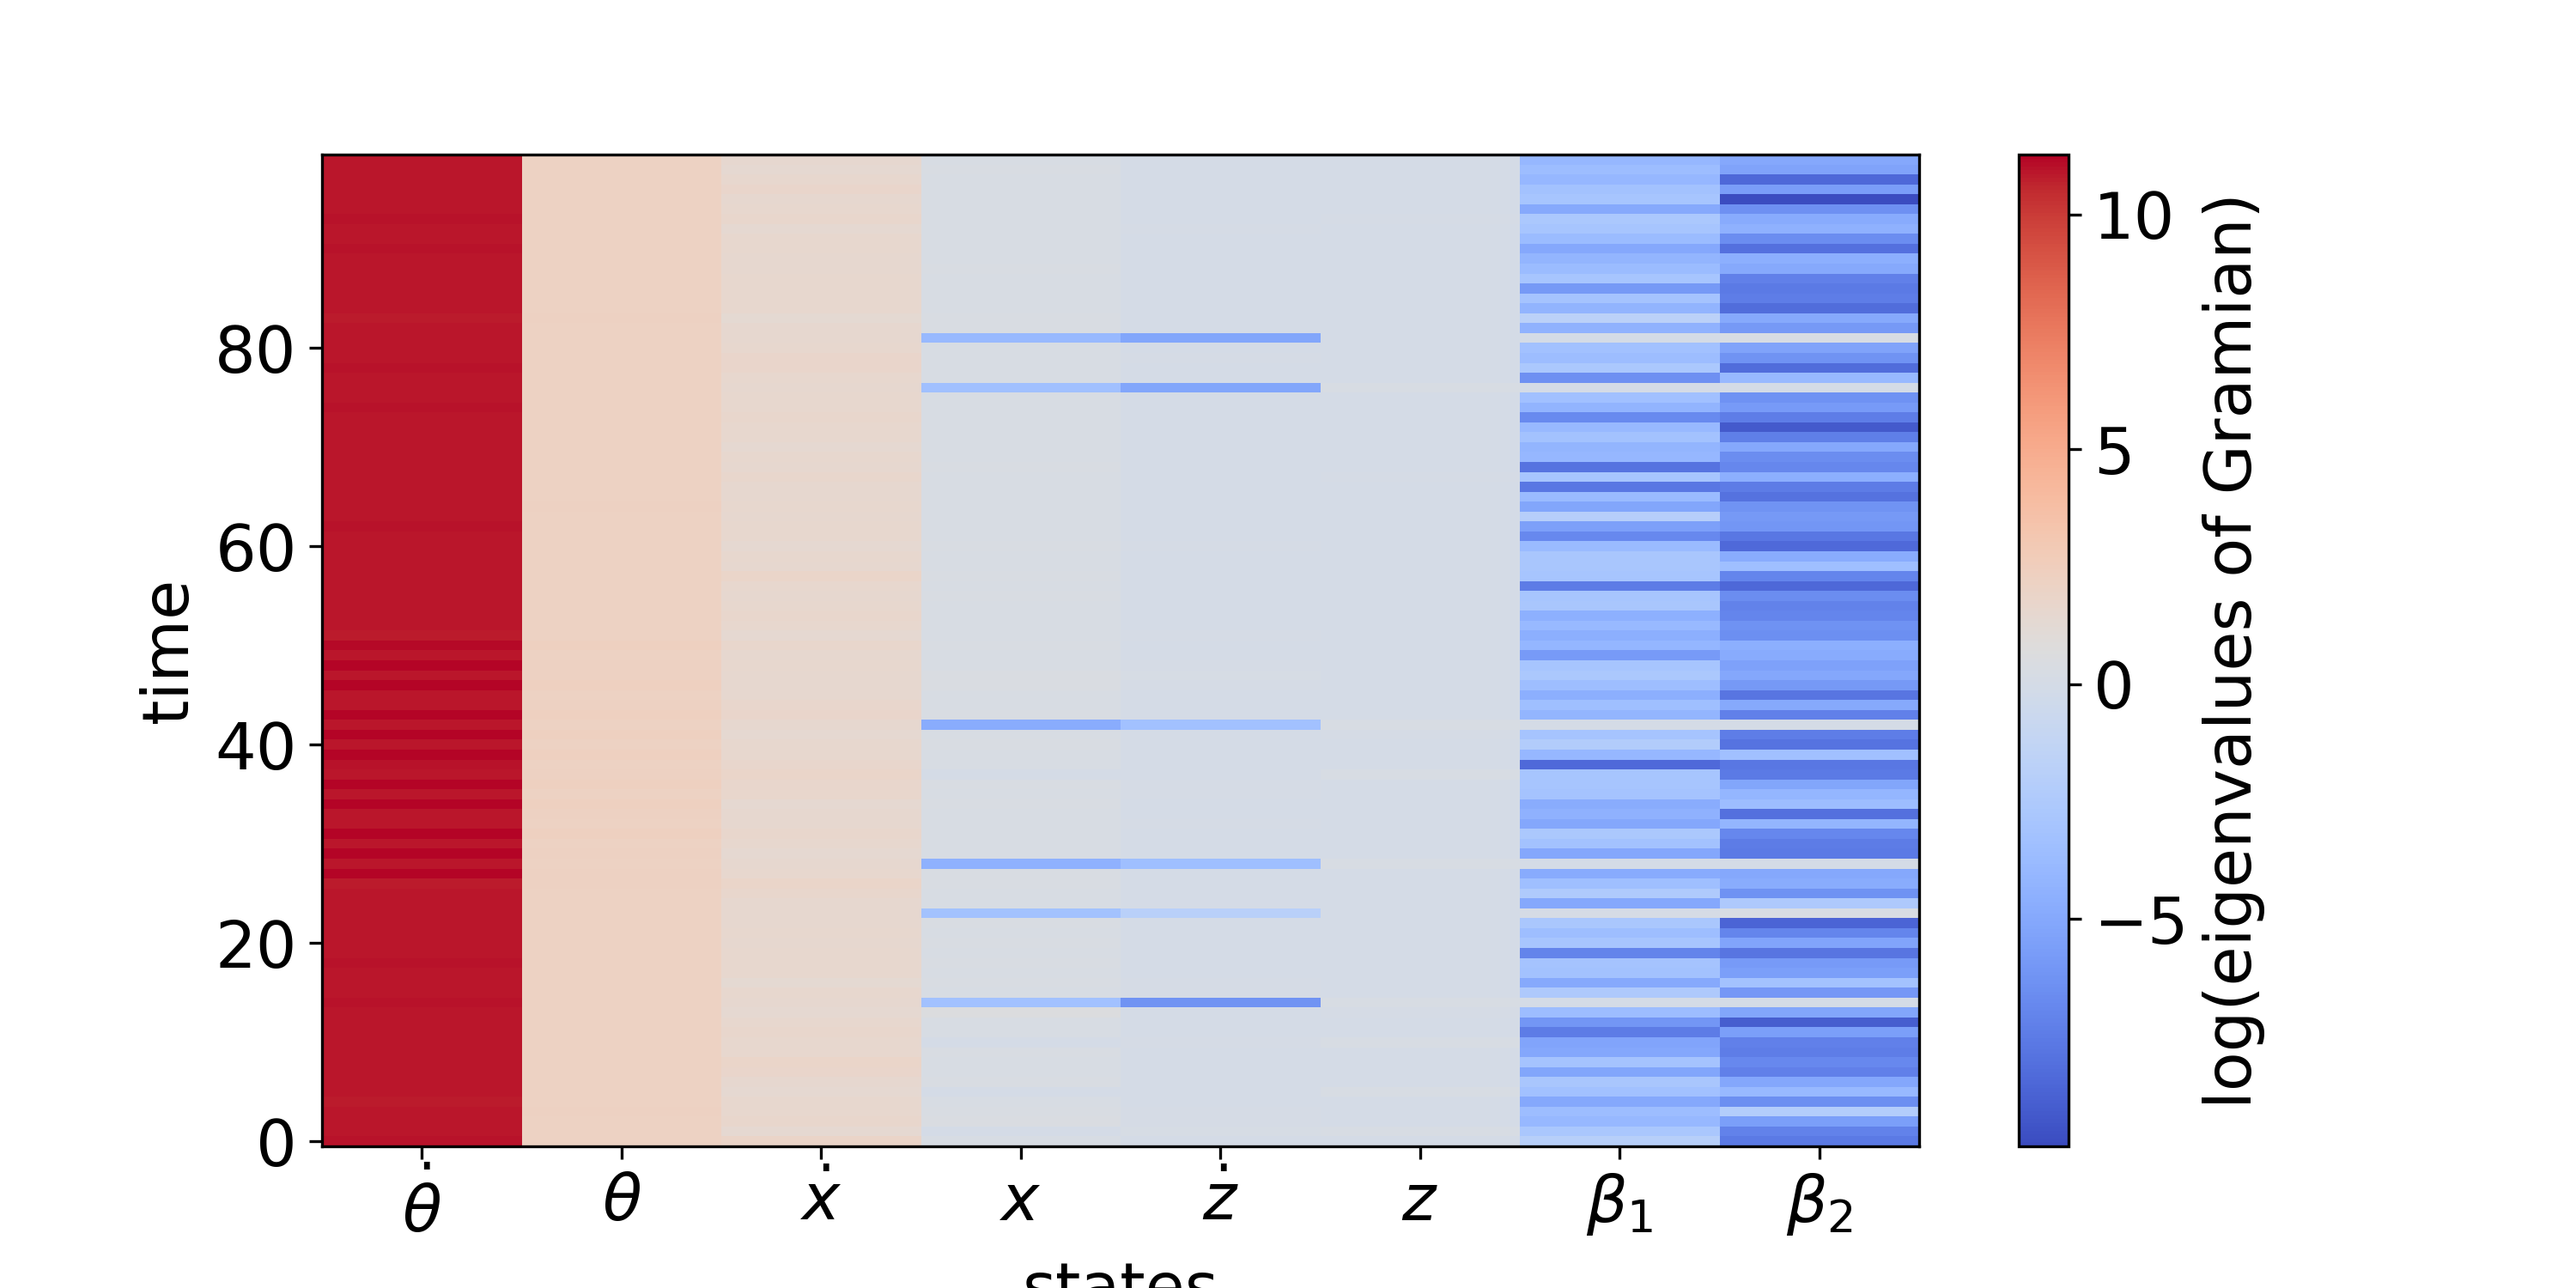
\includegraphics[width=15cm]{figures/gramian_eigenvalues_with_noisy_sinusoidal_x_and_h13.png}
        \caption{Eigenvalues of the Gramian matrix with time}
        \label{supfig:09c}
    \end{subfigure}
\end{figure}

\end{document}